\documentclass[12pt,a4paper]{article}

\usepackage[utf8]{inputenc}
\usepackage[T1]{fontenc}
\usepackage[french]{babel}
\usepackage{geometry}
\usepackage{setspace}
\usepackage{graphicx}
\usepackage{float}
\usepackage{array}
\usepackage{longtable}
\usepackage{booktabs}
\usepackage{xcolor}
\usepackage{listings}
\usepackage{hyperref}
\usepackage{enumitem}

\geometry{margin=2.5cm}
\setstretch{1.2}

\hypersetup{
    colorlinks=true,
    linkcolor=blue,
    urlcolor=blue,
    pdftitle={Rapport Academique VoIP - SIP/RTP},
    pdfauthor={Equipe Projet VoIP}
}

\lstset{
    basicstyle=\ttfamily\small,
    frame=single,
    breaklines=true,
    columns=fullflexible,
    keepspaces=true,
    showstringspaces=false
}

\title{\textbf{Rapport Académique\\Projet de Communication VoIP}}
\author{
AHOULIMI BIDENIMM \and SIDIKI ABOUBAKAR \\
EL KARFI SOUFIA \and LAZAAR EL MEHDI
}
\date{Avril 2026}

\begin{document}

\begin{titlepage}
    	\thispagestyle{empty}

    \begin{flushright}
        
\includegraphics[width=3.4cm]{../inpt.png}
    \end{flushright}

    \vspace*{0.8cm}

    \begin{center}
        {\Large\textbf{Institut National des Postes et Télécommunications}}\\[0.3cm]
        {\large\textbf{Filière : Smart ICT}}\\[1.6cm]

        {\LARGE\textbf{Rapport :}}\\[0.4cm]
        {\Large\textbf{Projet de Communication VoIP}}\\[1.1cm]

        \rule{0.9\textwidth}{0.8pt}\\[0.35cm]
        {\large\textbf{Sujet : Implémentation d'une solution VoIP basée sur SIP/RTP}}\\[0.35cm]
        \rule{0.9\textwidth}{0.8pt}\\[1.2cm]
    \end{center}

    \noindent
    \begin{tabular}{p{0.45\textwidth} p{0.5\textwidth}}
        	\textbf{Encadré par :} & \textbf{Travail effectué par :} \\
        Mr. Abdelali CHAOUB & AHOULIMI BIDENIMM \\
         & SIDIKI ABOUBAKAR \\
         & EL KARFI SOUFIA \\
         & LAZAAR EL MEHDI \\
    \end{tabular}

    \vfill

    \begin{center}
        \large Avril 2026
    \end{center}
\end{titlepage}

\newpage
\tableofcontents
\newpage

\section{Introduction}

La communication en temps réel sur Internet est devenue un composant fondamental des infrastructures numériques modernes. À mesure que les usages collaboratifs se multiplient (télétravail, visioconférence, assistance à distance, e-learning), les exigences en matière de latence, de qualité de service et d'interopérabilité se renforcent. Dans ce contexte, les technologies de Voice over IP (VoIP) occupent une place centrale, car elles permettent d'acheminer la voix via des réseaux IP tout en réduisant les coûts d'exploitation et en augmentant la flexibilité des architectures.

L'objectif de ce projet est de concevoir et implémenter une application VoIP académique complète, reposant sur les protocoles standards SIP (Session Initiation Protocol) pour la signalisation et RTP (Real-time Transport Protocol) pour le transport des flux audio. Le système développé adopte une architecture client-serveur où un serveur SIP joue les rôles de registrar et proxy, tandis que les clients assurent l'enregistrement, l'établissement des appels, la négociation des paramètres média (SDP) et la transmission audio bidirectionnelle.

D'un point de vue pédagogique, ce travail couvre plusieurs dimensions complémentaires :
\begin{itemize}[leftmargin=1.2cm]
    \item la compréhension des protocoles applicatifs de téléphonie sur IP ;
    \item la modélisation d'une architecture distribuée en environnement UDP ;
    \item l'implémentation logicielle en Python (socket, threading, gestion d'états) ;
    \item la validation expérimentale via des tests de connectivité et des scénarios d'appel.
\end{itemize}

Au-delà de la simple mise en relation de deux correspondants, le projet intègre une interface graphique utilisateur, une gestion de l'historique des appels, des contrôles de session (décrocher, refuser, raccrocher), ainsi qu'un support de traversal NAT via STUN pour améliorer la connectivité dans des contextes réseau réels. L'ensemble constitue une base solide pour l'étude des systèmes de communication multimédia temps réel.

Ce rapport présente, dans une démarche académique structurée, (i) un rappel historique de l'Internet et de WebRTC, (ii) une explication détaillée des protocoles SIP et RTP, (iii) les diagrammes d'architecture du système proposé, (iv) une section dédiée à l'interface fonctionnelle et aux captures d'écran, et (v) les tests réalisés avec leurs résultats. L'objectif final est de démontrer la cohérence entre conception, implémentation et validation, tout en identifiant les limites et perspectives d'évolution (ICE/TURN, sécurité média, scalabilité serveur).

\section{Historique : Internet et WebRTC}

\subsection{Évolution d'Internet}

L'histoire d'Internet peut être lue comme la progression d'un réseau de transport de données vers une plateforme de communication universelle. ARPANET (1969) introduit le principe de commutation de paquets : plutôt que de réserver un circuit dédié, les données sont fragmentées et acheminées dynamiquement. Cette rupture technologique constitue la base des communications modernes, y compris la voix sur IP.

Dans les années 1980, la standardisation TCP/IP (adoption officielle sur ARPANET en 1983) permet l'interconnexion de réseaux hétérogènes. Le modèle en couches favorise l'évolution indépendante des services applicatifs : SMTP pour le mail, FTP pour le transfert de fichiers, puis HTTP pour le Web. Avec la démocratisation du World Wide Web dans les années 1990, Internet devient une infrastructure globale orientée grand public.

La décennie 2000 marque le passage d'un Internet principalement asynchrone (pages Web, e-mail) vers un Internet interactif. Les besoins de communication en temps réel augmentent fortement : téléphonie logicielle, centres d'appels IP, visioconférence, travail collaboratif. Or, la voix et la vidéo imposent des contraintes techniques strictes :
\begin{itemize}[leftmargin=1.2cm]
    \item latence faible (idéalement < 150 ms aller simple),
    \item gigue maîtrisée (variation du délai inter-paquets),
    \item tolérance limitée aux pertes,
    \item adaptation aux environnements NAT/pare-feu.
\end{itemize}

Cette évolution motive l'adoption d'une pile protocolaire spécialisée : SIP pour la signalisation, SDP pour la description média, RTP/RTCP pour le transport et la supervision temps réel.

\subsection{De la VoIP classique aux architectures temps réel modernes}

Avant WebRTC, les architectures VoIP reposaient sur des clients dédiés (softphones, IP phones) connectés à des serveurs SIP/IMS/PBX. Les défis majeurs étaient déjà présents : négociation des codecs, interopérabilité multi-constructeurs, sécurité de la signalisation, et traversal NAT via STUN/TURN/ALG. Les solutions étaient efficaces mais souvent complexes à déployer dans des environnements hétérogènes.

Progressivement, les mécanismes de qualité de service (priorisation DiffServ, buffers de gigue, adaptation de débit) et de sécurité (SIP over TLS, SRTP) se sont imposés dans les déploiements professionnels. Cette maturation de la VoIP classique a préparé le terrain aux communications temps réel intégrées au navigateur.

\subsection{Historique de WebRTC}

WebRTC (Web Real-Time Communication), lancé autour de 2011 (Google puis normalisation W3C/IETF), vise à rendre la communication audio/vidéo et data-channel accessible directement depuis le navigateur, sans plugin. L'apport principal est l'intégration native des briques historiquement séparées dans la VoIP : connectivité réseau, sécurité, codecs, et API applicatives.

WebRTC ne remplace pas les principes fondamentaux de la VoIP ; il les encapsule dans un cadre standardisé orienté Web, notamment via :
\begin{itemize}[leftmargin=1.2cm]
    \item \textbf{ICE} (Interactive Connectivity Establishment) : découverte et sélection du meilleur chemin réseau,
    \item \textbf{STUN/TURN} : traversal NAT et relais en cas d'échec du pair-à-pair,
    \item \textbf{DTLS-SRTP} : chiffrement et authentification des flux média,
    \item \textbf{API JavaScript} normalisées (\texttt{getUserMedia}, \texttt{RTCPeerConnection}, \texttt{RTCDataChannel}).
\end{itemize}

Sur le plan architectural, WebRTC réutilise des concepts proches de SIP/RTP (signalisation séparée du média, SDP-like offer/answer, transport RTP sécurisé). La différence est que la signalisation WebRTC est volontairement laissée à l'application (WebSocket, SIP over WebSocket, etc.), alors que SIP définit explicitement les méthodes et transactions.

Dans ce projet, l'approche retenue est SIP/RTP classique (hors navigateur), mais l'intégration de STUN côté client rapproche l'implémentation des contraintes réelles d'Internet public. Cette continuité permet d'articuler clairement les fondements académiques de la VoIP et les pratiques contemporaines issues de WebRTC.

\section{Explication des protocoles SIP et RTP}

\subsection{SIP : signalisation des sessions}

SIP (RFC 3261) est un protocole textuel de couche application, inspiré du paradigme requête/réponse. Son rôle est la \textbf{signalisation} des sessions : découverte du correspondant, négociation des paramètres multimédia, établissement et terminaison des appels. SIP ne transporte pas directement les données audio ; il pilote la session qui sera ensuite portée par RTP.

Dans une architecture SIP standard, plusieurs entités coopèrent :
\begin{itemize}[leftmargin=1.2cm]
    \item \textbf{User Agent Client (UAC)} : émet les requêtes (ex. INVITE),
    \item \textbf{User Agent Server (UAS)} : reçoit et répond,
    \item \textbf{Registrar} : gère l'enregistrement des utilisateurs,
    \item \textbf{Proxy} : relaie/routage des requêtes et réponses.
\end{itemize}

Le modèle SIP distingue des notions importantes :
\begin{itemize}[leftmargin=1.2cm]
    \item \textbf{Transaction} : unité requête/réponses associées,
    \item \textbf{Dialogue} : relation SIP persistante entre deux UA (identifiée par Call-ID + tags),
    \item \textbf{Session} : échange média effectif (RTP).
\end{itemize}

\textbf{Méthodes principales utilisées dans le projet :}
\begin{itemize}[leftmargin=1.2cm]
    \item \texttt{REGISTER} : enregistrement d'un client au serveur SIP,
    \item \texttt{INVITE} : initiation d'appel,
    \item \texttt{ACK} : confirmation d'une réponse finale positive,
    \item \texttt{BYE} : fin d'appel actif,
    \item \texttt{CANCEL} : annulation d'appel en cours d'établissement,
    \item \texttt{OPTIONS} : test de disponibilité/capacité.
\end{itemize}

	extbf{Codes de réponse clés :} 100 (Trying), 180 (Ringing), 200 (OK), 404 (Not Found), 480 (Temporarily Unavailable), 603 (Decline).

\subsection{Structure des messages SIP et champs critiques}

Les messages SIP incluent des en-têtes déterminants pour la cohérence protocolaire :
\begin{itemize}[leftmargin=1.2cm]
    \item \texttt{Via} : traçabilité du chemin de signalisation ;
    \item \texttt{From}/\texttt{To} : identités logique appelant/appelé ;
    \item \texttt{Call-ID} : identifiant global d'appel ;
    \item \texttt{CSeq} : séquencement des requêtes dans un dialogue ;
    \item \texttt{Contact} : adresse de retour directe de l'UA ;
    \item \texttt{Content-Type}/\texttt{Content-Length} : gestion du corps SDP.
\end{itemize}

Dans l'implémentation du projet, la robustesse de ces champs est essentielle : un \texttt{Call-ID} stable et un \texttt{CSeq} cohérent garantissent la corrélation correcte des réponses, tandis que les informations SDP assurent l'établissement de la session média.

\subsection{Cycle d'appel SIP dans le projet}

Le scénario nominal suit les étapes suivantes :
\begin{enumerate}[leftmargin=1.2cm]
    \item \textbf{REGISTER} de chaque client auprès du serveur ;
    \item \textbf{INVITE} de l'appelant avec offre SDP ;
    \item réponses provisoires \textbf{100 Trying} puis \textbf{180 Ringing} ;
    \item réponse finale \textbf{200 OK} avec SDP de l'appelé ;
    \item \textbf{ACK} de confirmation ;
    \item démarrage du flux \textbf{RTP} bidirectionnel ;
    \item terminaison par \textbf{BYE} (appel actif) ou \textbf{CANCEL} (appel non établi).
\end{enumerate}

Le projet gère explicitement la distinction \texttt{CANCEL} vs \texttt{BYE}, ce qui est fondamental pour un comportement utilisateur correct (annuler un appel en sonnerie n'est pas équivalent à terminer un appel actif).

\subsection{RTP : transport des flux audio}

RTP (RFC 3550) transporte les données audio en temps réel, généralement sur UDP. Le protocole est conçu pour minimiser la latence et tolérer des pertes modérées, contrairement aux mécanismes de retransmission typiques de TCP.

Les champs principaux du header RTP ont un rôle opérationnel direct :
\begin{itemize}[leftmargin=1.2cm]
    \item \textbf{Sequence Number} : détection de pertes et réordonnancement,
    \item \textbf{Timestamp} : restitution temporelle des paquets,
    \item \textbf{Payload Type} : identification du codec,
    \item \textbf{SSRC} : identification de la source média.
\end{itemize}

Le récepteur utilise ces informations avec un \emph{jitter buffer} implicite (ou logique équivalente) pour lisser les variations inter-paquets. La qualité perçue dépend alors d'un compromis entre latence supplémentaire et stabilité audio.

Dans cette implémentation, le flux audio est encodé principalement en G.711 (PCMU/PCMA), avec un framing de 20 ms (160 échantillons à 8 kHz), ce qui correspond à 50 paquets RTP par seconde.

\subsection{Qualité de service et limites pratiques}

Même en réseau local, les communications temps réel sont sensibles à :
\begin{itemize}[leftmargin=1.2cm]
    \item la \textbf{latence} (délai de bout en bout),
    \item la \textbf{gigue} (variation de latence),
    \item les \textbf{pertes de paquets},
    \item les \textbf{asymétries NAT} dans les contextes Internet.
\end{itemize}

Le projet intègre STUN pour améliorer l'annonce d'endpoint public RTP. Toutefois, dans les cas de NAT symétrique ou politiques firewall strictes, un relais TURN et une négociation ICE complète deviennent nécessaires pour garantir la connectivité de bout en bout.

\subsection{Rôle de SDP}

SDP (RFC 4566) encapsule les paramètres techniques de la session média. Dans ce projet, il est transporté dans les messages SIP (INVITE/200 OK) et contient au minimum :
\begin{itemize}[leftmargin=1.2cm]
    \item l'adresse IP et le port RTP (
	exttt{c=} et \texttt{m=audio}),
    \item les codecs proposés (
	exttt{a=rtpmap}),
    \item le mode de transmission (
	exttt{a=sendrecv}/\texttt{recvonly}).
\end{itemize}

La négociation suit une logique \emph{offer/answer} : l'appelant propose un ensemble de codecs, l'appelé sélectionne un sous-ensemble compatible. Cette étape conditionne directement la compatibilité média et la réussite de l'appel.

\subsection{Extraits de code d'implémentation des protocoles}

Cette sous-section présente des extraits représentatifs du code réellement utilisé dans le projet pour chaque protocole principal.

\subsubsection{Implémentation SIP (construction et sérialisation des messages)}

\begin{lstlisting}[language=Python,caption={Sérialisation d'un message SIP (\texttt{src/shared/sip\_messages.py})}]
@dataclass
class SIPMessage:
    method: str = ""
    uri: str = ""
    headers: Dict[str, str] = field(default_factory=dict)
    body: str = ""

    def to_bytes(self) -> bytes:
        lines: List[str] = []

        if self.method:
            first_line = f"{self.method} {self.uri} SIP/2.0"
        else:
            status = self.headers.get('Status', '200 OK').strip()
            if status and status.split()[0].isdigit() and len(status.split()) == 1:
                status = f"{status} OK"
            first_line = f"SIP/2.0 {status}"

        lines.append(first_line)
        body_bytes = self.body.encode('utf-8') if self.body else b''
        self.headers['Content-Length'] = str(len(body_bytes))

        for header, value in self.headers.items():
            lines.append(f"{header}: {value}")

        lines.append("")
        if self.body:
            lines.append(self.body)

        return "\r\n".join(lines).encode('utf-8')
\end{lstlisting}
\newpage
\subsubsection{Implémentation SDP (offre/réponse et parsing)}

\begin{lstlisting}[language=Python,caption={Création et parsing SDP (\texttt{src/shared/sip\_messages.py})}]
def create_sdp(offer: bool, ip: str, port: int, codecs: List[str] = None) -> str:
    if codecs is None:
        codecs = ['PCMU', 'PCMA']

    codec_payload_types = {'PCMU': 0, 'PCMA': 8, 'opus': 123}
    session_id = random.randint(1000, 9999)

    sdp_lines = [
        "v=0",
        f"o=- {session_id} {session_id} IN IP4 {ip}",
        "s=-",
        "c=IN IP4 " + ip,
        "t=0 0",
        "m=audio " + str(port) + " RTP/AVP " + " ".join(str(codec_payload_types.get(c, 123)) for c in codecs),
        "a=rtpmap:0 PCMU/8000",
        "a=rtpmap:8 PCMA/8000",
        "a=rtpmap:123 opus/48000/2",
        "a=sendrecv" if offer else "a=recvonly"
    ]
    return "\r\n".join(sdp_lines)

def parse_sdp(sdp_body: str) -> Dict:
    result = {'ip': '', 'port': 0, 'codecs': []}
    for raw_line in sdp_body.split('\r\n'):
        line = raw_line.strip()
        if line.startswith('c=IN IP4 '):
            parts = line.split()
            if len(parts) >= 3:
                result['ip'] = parts[2]
        elif line.startswith('m=audio '):
            parts = line.split()
            if len(parts) >= 2 and parts[1].isdigit():
                result['port'] = int(parts[1])
        elif line.startswith('a=rtpmap:'):
            parts = line.split()
            if len(parts) >= 2:
                encoding = parts[1].split('/')[0].strip()
                if encoding and encoding not in result['codecs']:
                    result['codecs'].append(encoding)
    return result
\end{lstlisting}

\subsubsection{Implémentation RTP (encapsulation et émission des paquets)}

\begin{lstlisting}[language=Python,caption={Paquet RTP et envoi audio (\texttt{src/shared/rtp.py})}]
@dataclass
class RTPPacket:
    version: int = 2
    payload_type: int = 0
    sequence_number: int = 0
    timestamp: int = 0
    ssrc: int = 0
    payload: bytes = b''

    def to_bytes(self) -> bytes:
        first_byte = (self.version << 6)
        second_byte = self.payload_type
        header = struct.pack('!BBHII', first_byte, second_byte,
                             self.sequence_number,
                             self.timestamp & 0xFFFFFFFF,
                             self.ssrc)
        return header + self.payload

class RTPSession:
    def send_audio_frame(self, audio_data: bytes, marker: bool = False) -> bool:
        if not self.socket or not self.remote_addr:
            return False

        self.timestamp = (self.timestamp + 160) & 0xFFFFFFFF
        packet = RTPPacket(
            version=2,
            payload_type=self.payload_type,
            sequence_number=self.sequence_number & 0xFFFF,
            timestamp=self.timestamp,
            ssrc=self.ssrc,
            marker=1 if marker else 0,
            payload=audio_data
        )
        self.socket.sendto(packet.to_bytes(), self.remote_addr)
        self.sequence_number += 1
        return True
\end{lstlisting}

\subsubsection{Implémentation STUN (découverte d'endpoint public UDP)}

\begin{lstlisting}[language=Python,caption={Client STUN minimal (\texttt{src/shared/stun.py})}]
MAGIC_COOKIE = 0x2112A442
BINDING_REQUEST = 0x0001
BINDING_SUCCESS_RESPONSE = 0x0101
XOR_MAPPED_ADDRESS = 0x0020

def get_stun_mapped_address(
    udp_socket: socket.socket,
    stun_host: str,
    stun_port: int = 19302,
    timeout: float = 1.5,
) -> Optional[Tuple[str, int]]:
    request, tx_id = _build_binding_request()
    previous_timeout = udp_socket.gettimeout()
    try:
        udp_socket.settimeout(timeout)
        udp_socket.sendto(request, (stun_host, stun_port))
        data, _ = udp_socket.recvfrom(2048)

        msg_type, msg_len, cookie, rx_tx_id = struct.unpack("!HHI12s", data[:20])
        if msg_type != BINDING_SUCCESS_RESPONSE:
            return None
        if cookie != MAGIC_COOKIE or rx_tx_id != tx_id:
            return None

        # Parse attributes until XOR-MAPPED-ADDRESS
        # ...
        return parsed
    finally:
        udp_socket.settimeout(previous_timeout)
\end{lstlisting}
\newpage
\subsubsection{Gestion d'état d'appel SIP (CANCEL vs BYE)}

\begin{lstlisting}[language=Python,caption={Terminaison d'appel selon l'état (\texttt{src/client/sip\_client.py})}]
def hangup(self):
    if not self.current_call:
        return

    call_status = self.current_call.status
    method = 'CANCEL' if call_status in ('initiating', 'ringing') else 'BYE'

    builder = SIPRequestBuilder(method, f'sip:{self.current_call.remote_user}@{self.server_host}')
    builder.call_id = self.current_call.call_id
    builder.from_tag = self.user_id
    builder.add_header('Via', f"SIP/2.0/UDP {self._get_local_ip()};branch={generate_via_branch()}")

    request = builder.build()
    self.sip_socket.sendto(request.to_bytes(), (self.server_host, self.server_port))
\end{lstlisting}

\section{Diagrammes d'architecture}

\subsection{Architecture client-serveur}

\begin{figure}[H]
\centering
\begin{lstlisting}
Client A (SIP UA)  <------ SIP ------>  Serveur SIP/Proxy  <------ SIP ------>  Client B (SIP UA)
       |                                                                                  |
       +----------------------------- RTP Audio Bidirectionnel ----------------------------+
\end{lstlisting}
\caption{Architecture logique client-serveur et chemin des flux.}
\end{figure}

\subsection{Flux d'un appel et médias RTP}

\begin{figure}[H]
\centering
\begin{lstlisting}
Client A                     Serveur SIP                     Client B
   |------ REGISTER ------->|                                  |
   |<------ 200 OK ---------|                                  |
   |------ INVITE --------->|                                  |
   |<----- 100 Trying ------|                                  |
   |                        |------ INVITE ------------------->|
   |                        |<----- 180 Ringing ---------------|
   |<----- 180 Ringing -----|                                  |
   |                        |<----- 200 OK --------------------|
   |<------ 200 OK ---------|                                  |
   |------ ACK -----------> |                                  |
   |                        |------ ACK ---------------------->|
   |<======================== RTP STREAM ======================>|
   |------ BYE -----------> |                                  |
   |<------ 200 OK ---------|                                  |
\end{lstlisting}
\caption{Séquence simplifiée SIP + établissement du flux RTP.}
\end{figure}

\section{Capture d'écran de l'application fonctionnelle}
Etape 1 : Lancement du serveur SIP (terminal dédié) \\

\begin{figure}[H]
\centering
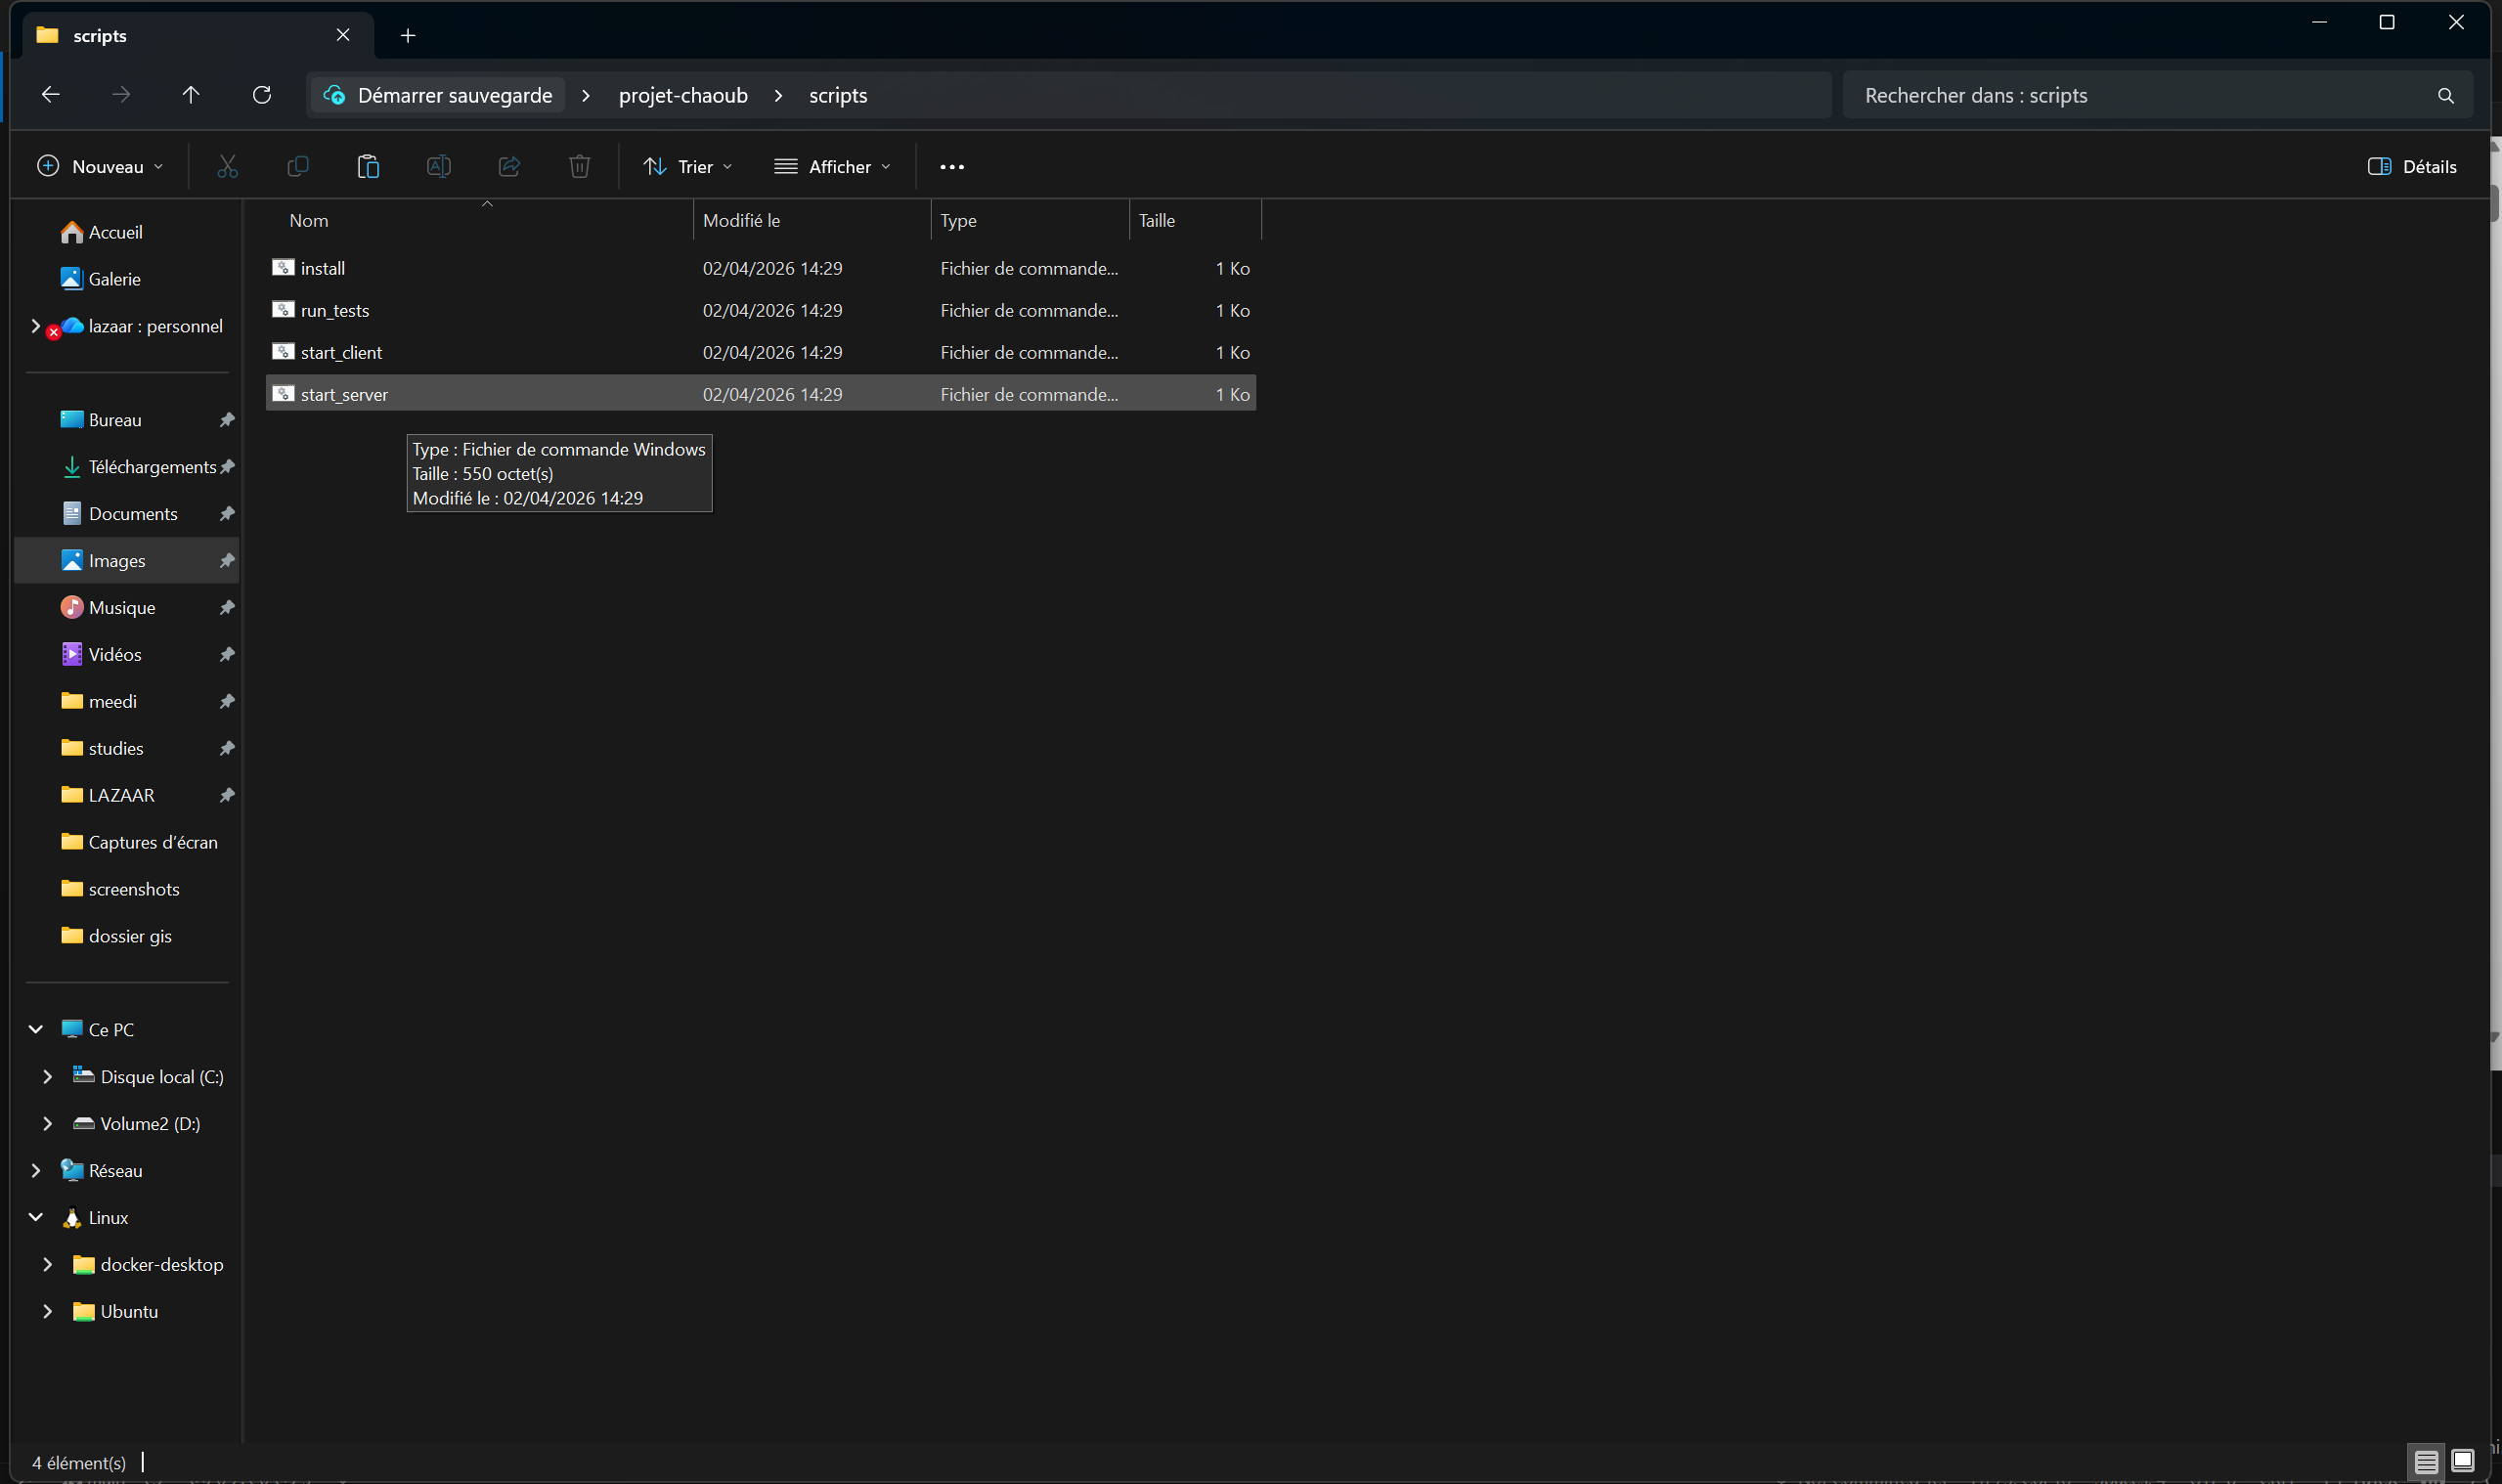
\includegraphics[width=0.8\textwidth]{screenshots/sc1.png}
\end{figure}
\begin{figure}[H]
\centering
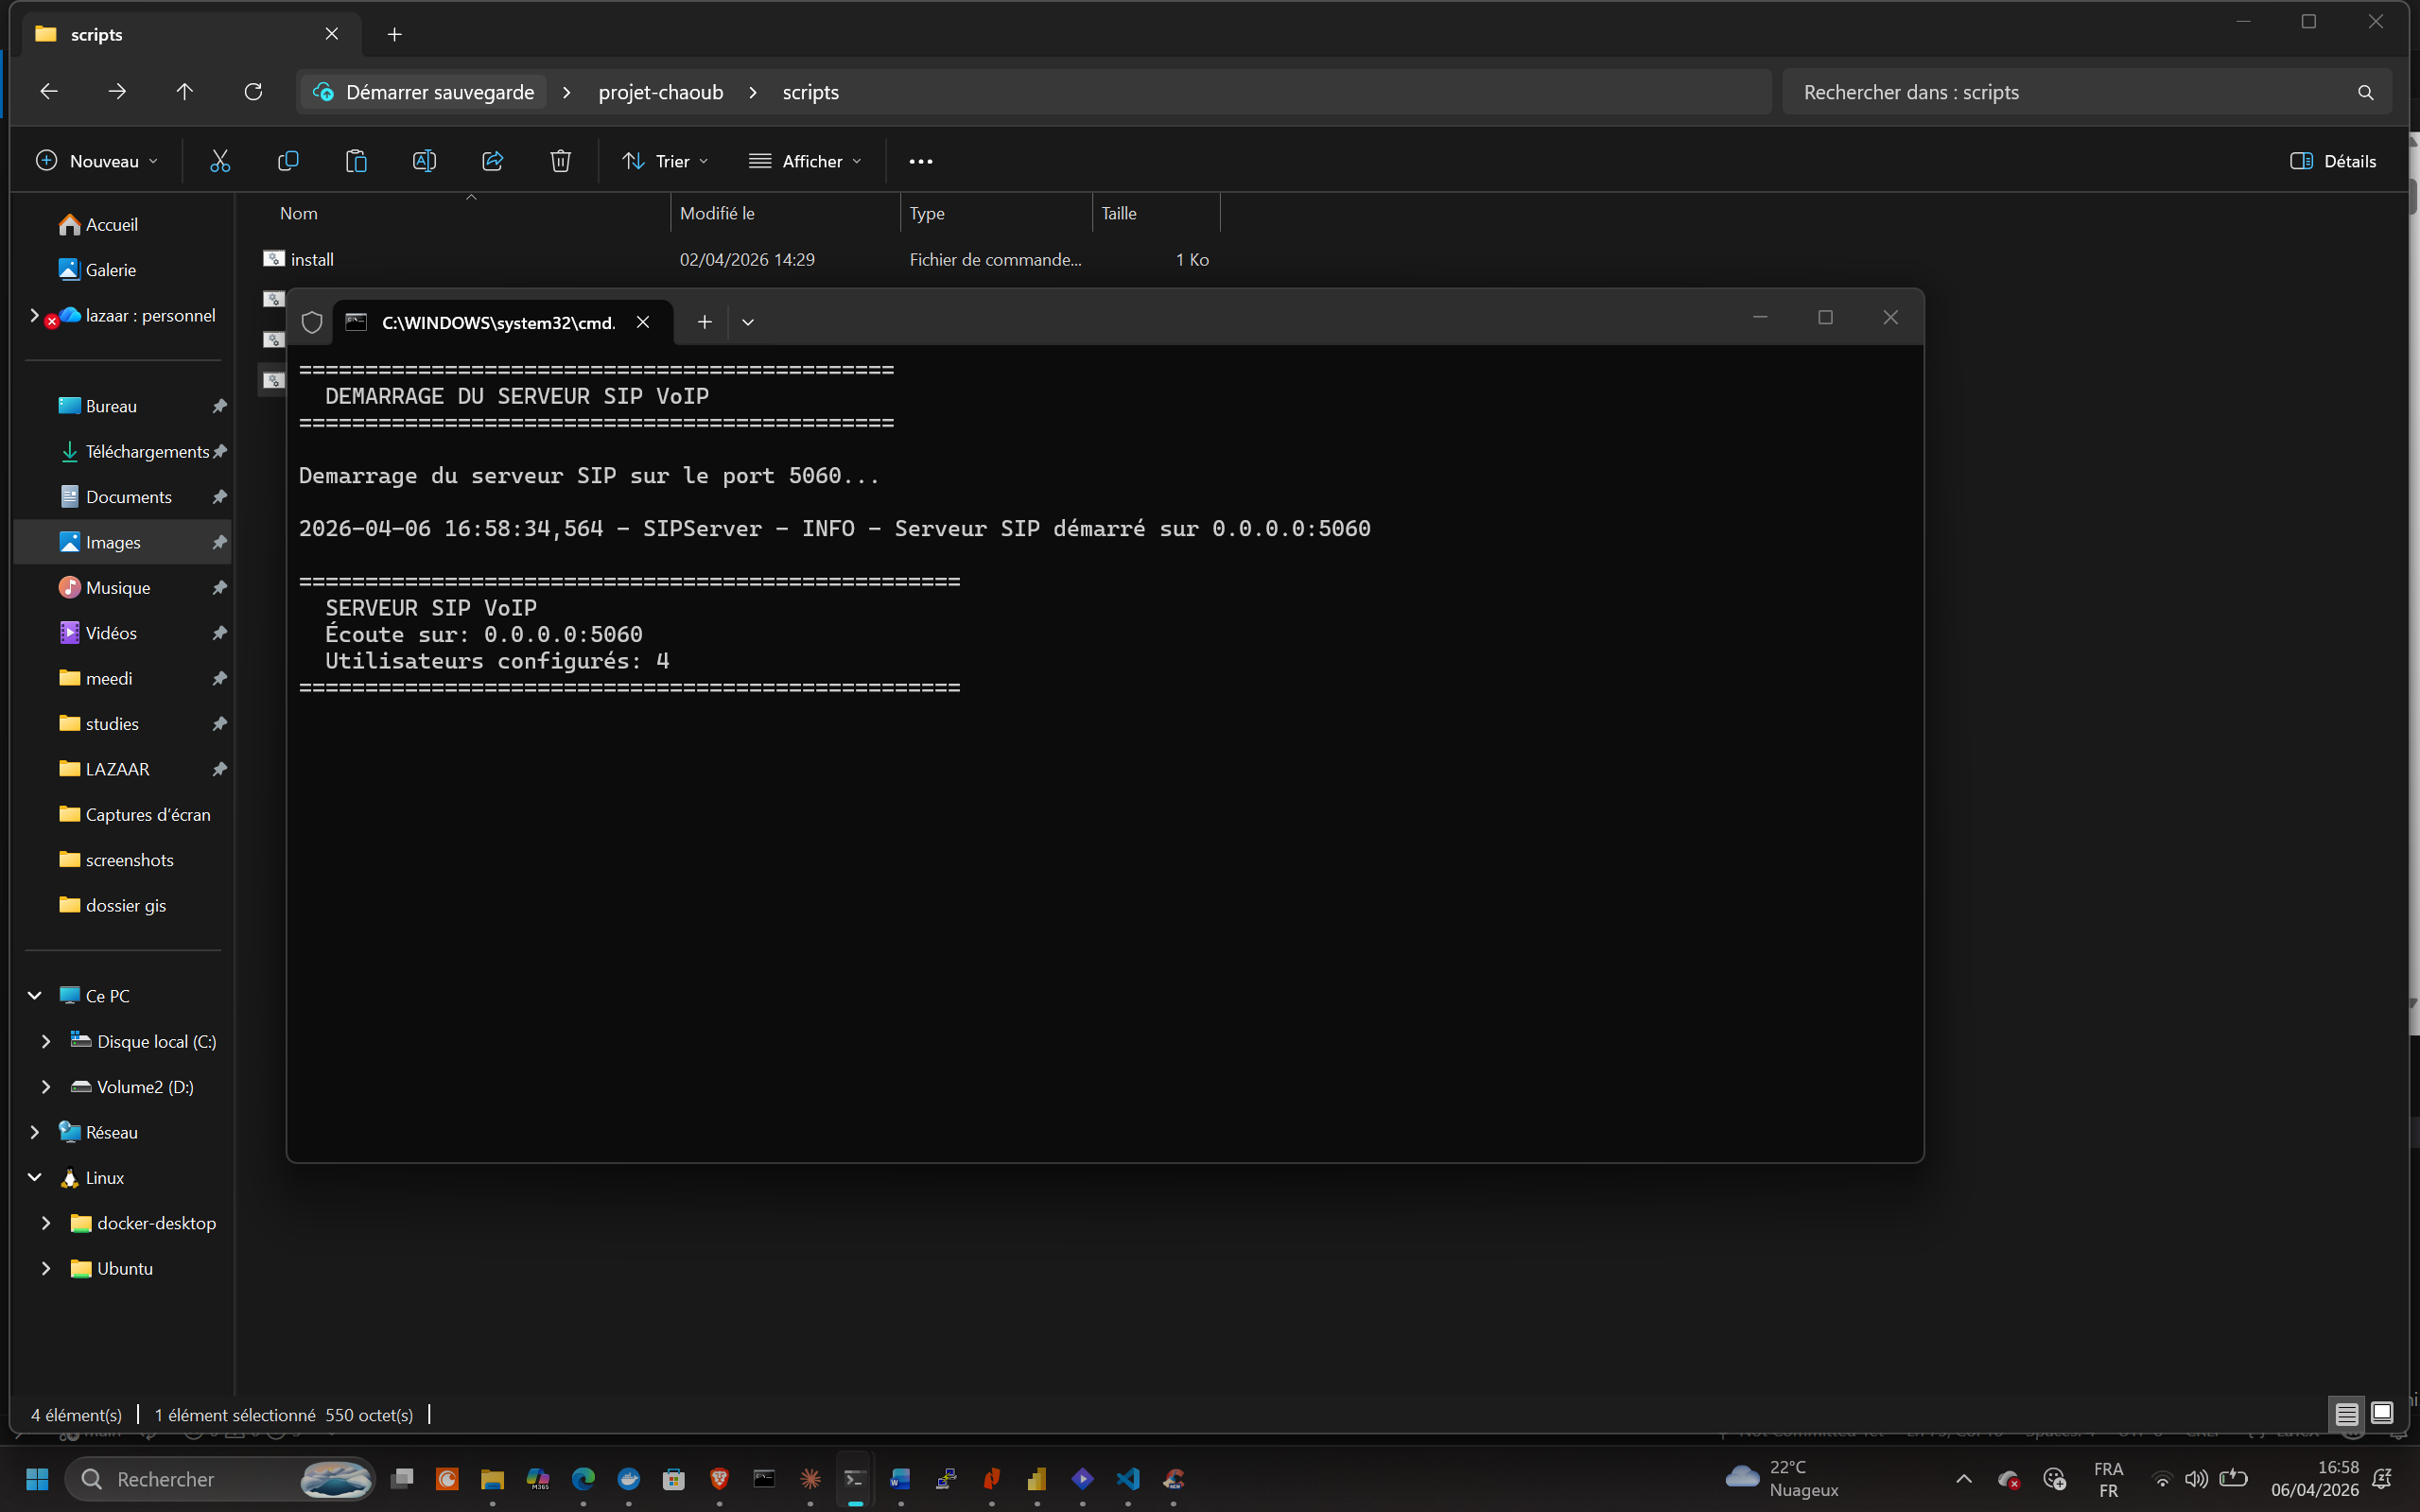
\includegraphics[width=0.8\textwidth]{screenshots/sc2.png}
\end{figure}
Etape 2 : Lancement des clients et enregistrement \\
\begin{figure}[H]
\centering
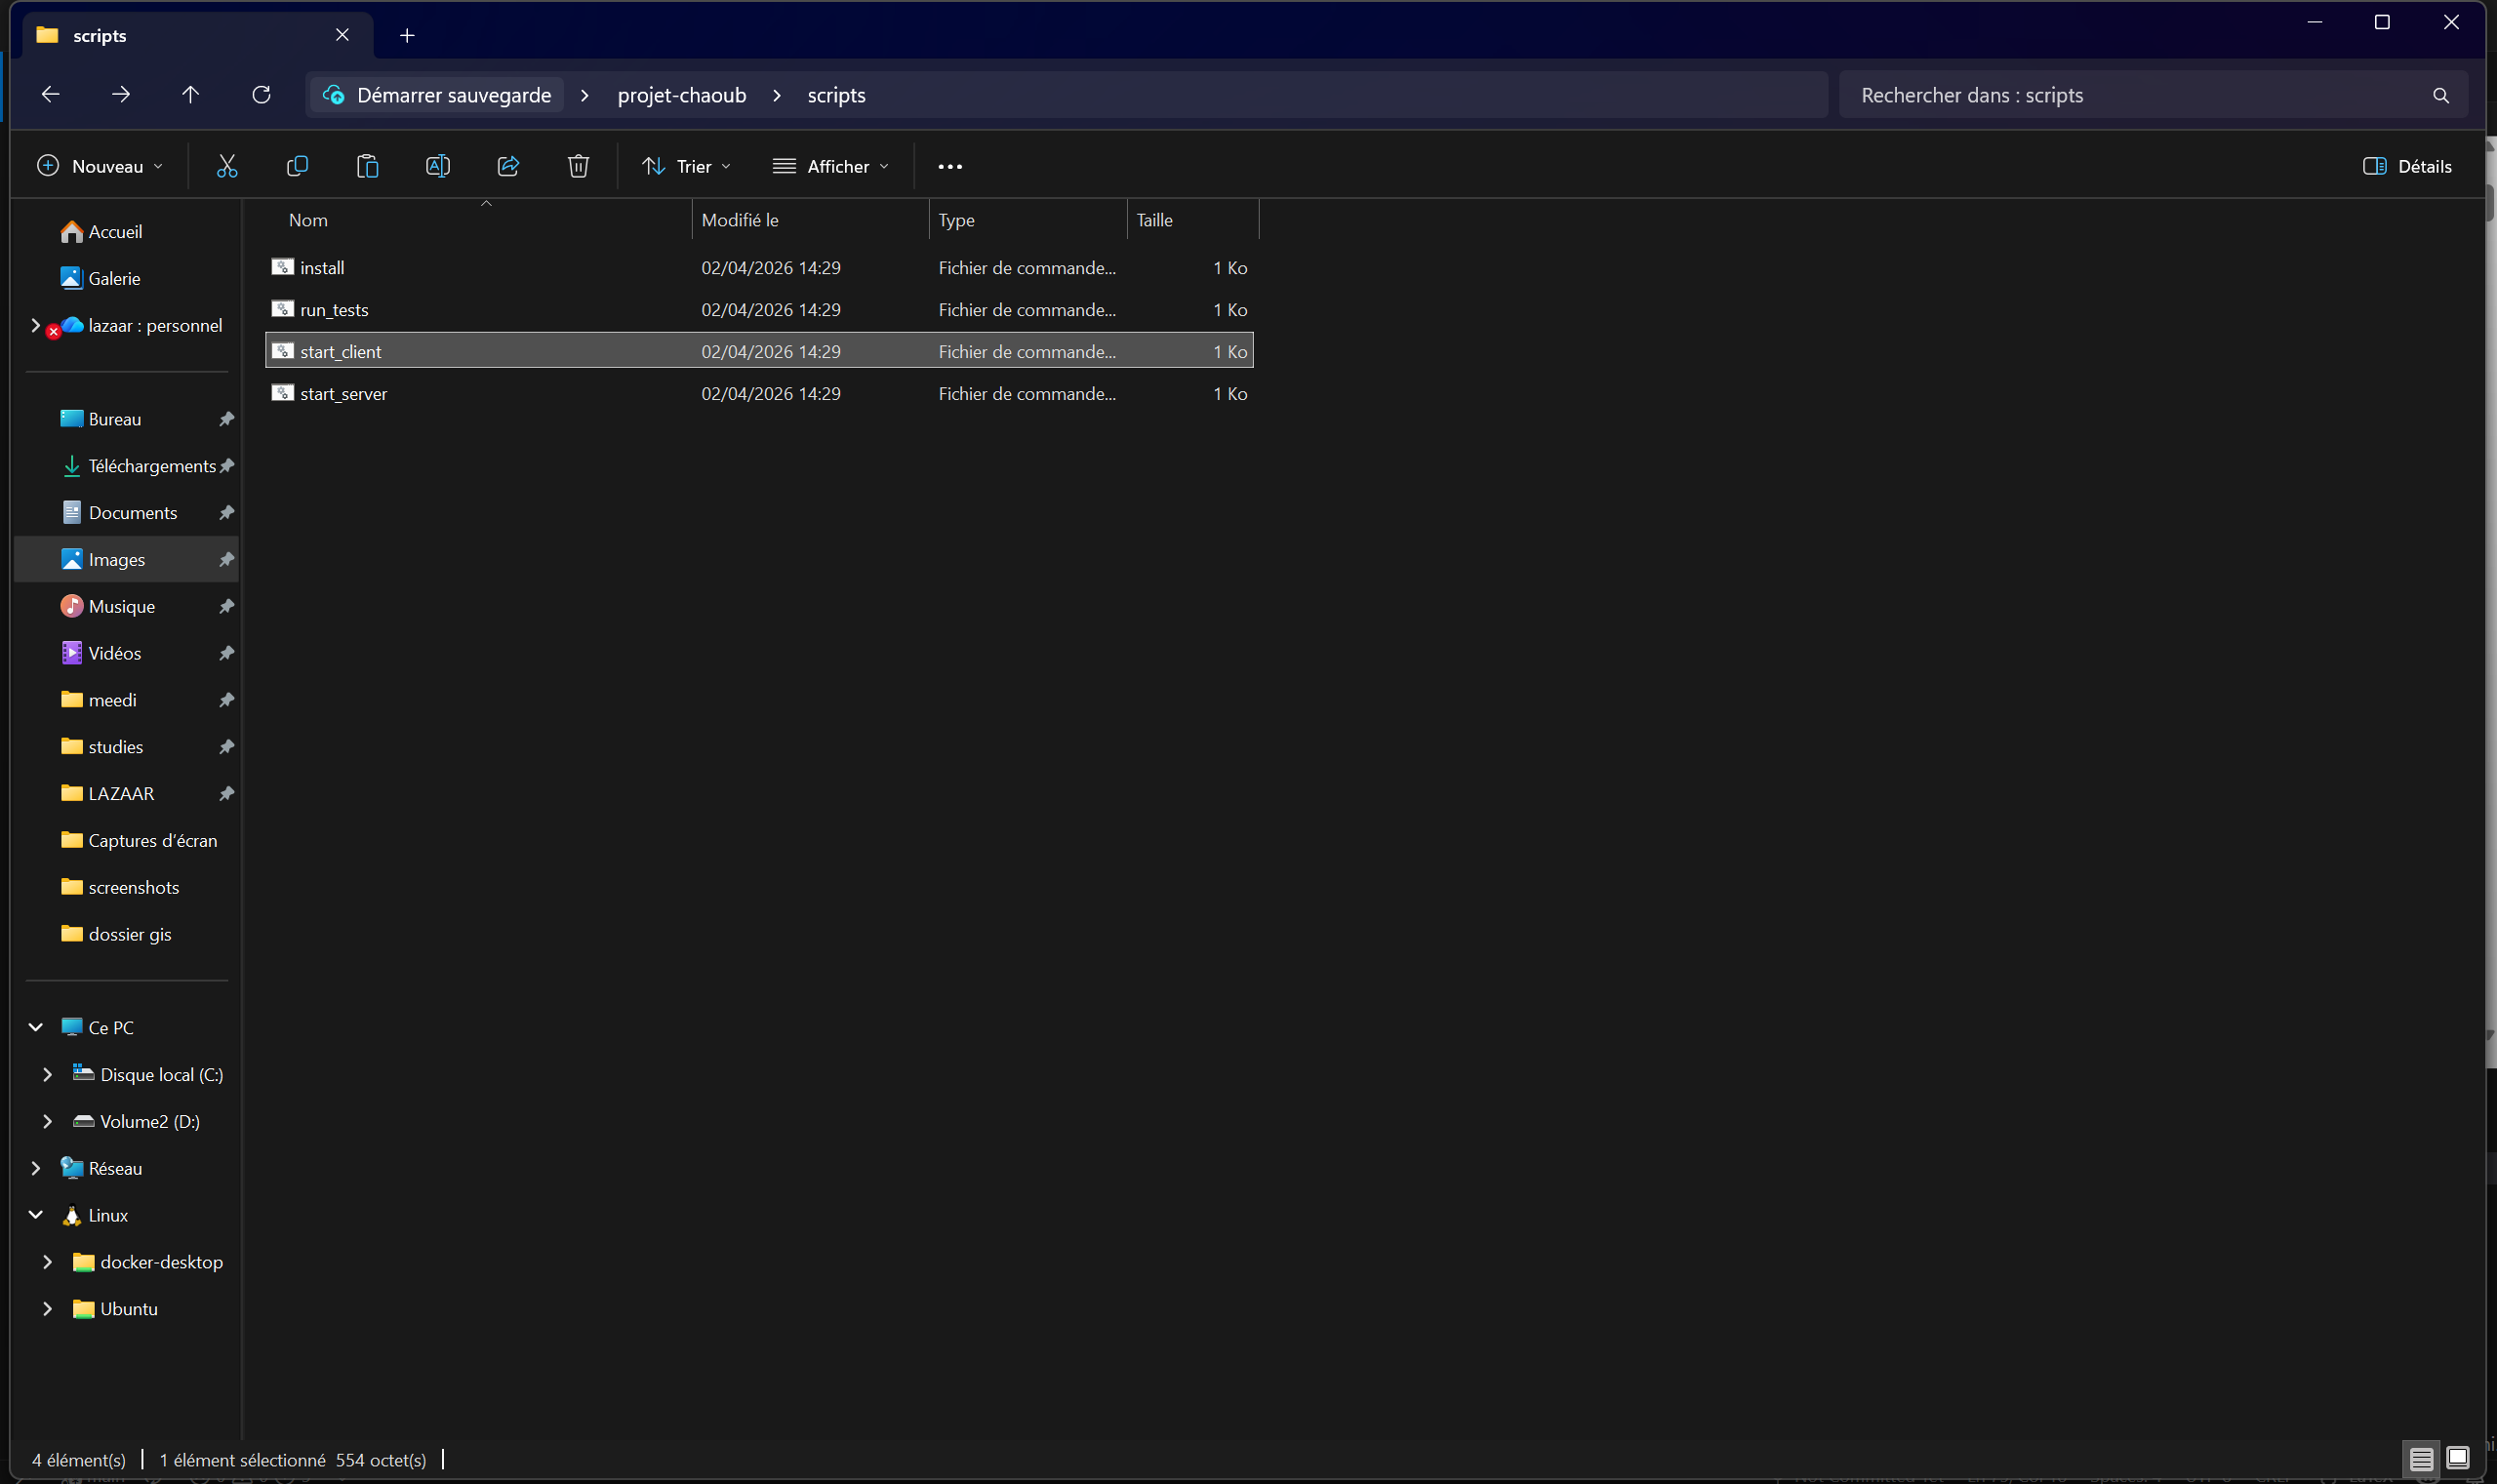
\includegraphics[width=0.8\textwidth]{screenshots/sc3.png}
\end{figure}
\begin{figure}[H]
\centering
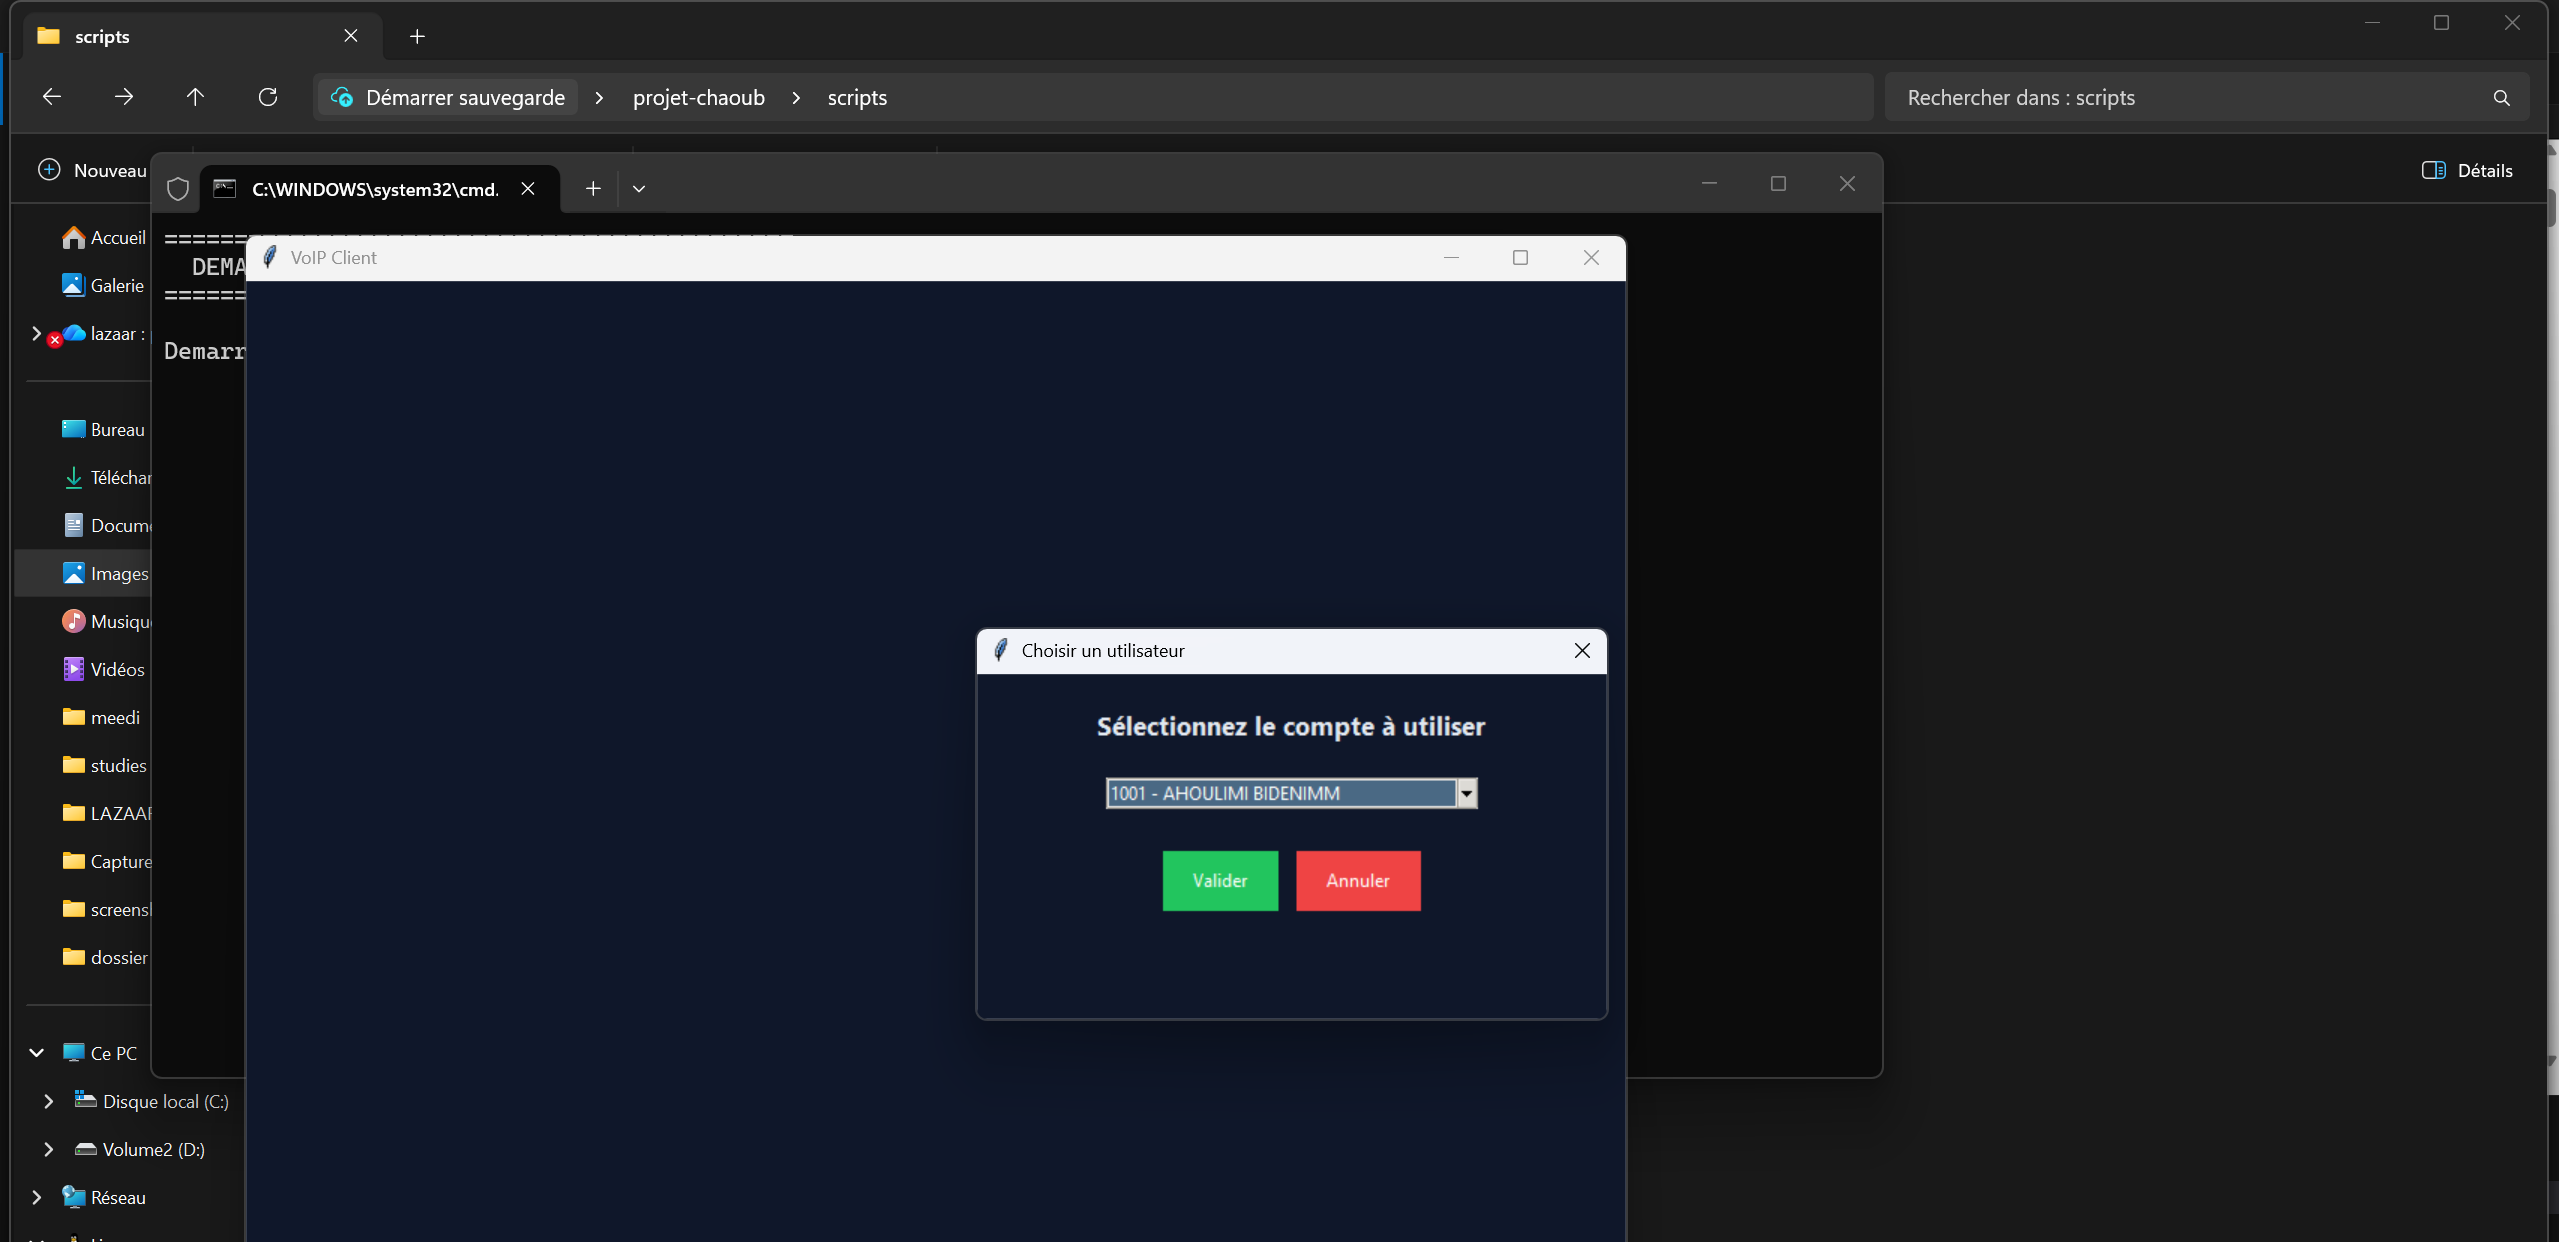
\includegraphics[width=0.8\textwidth]{screenshots/sc4.png}
\end{figure}
\begin{figure}[H]
\centering
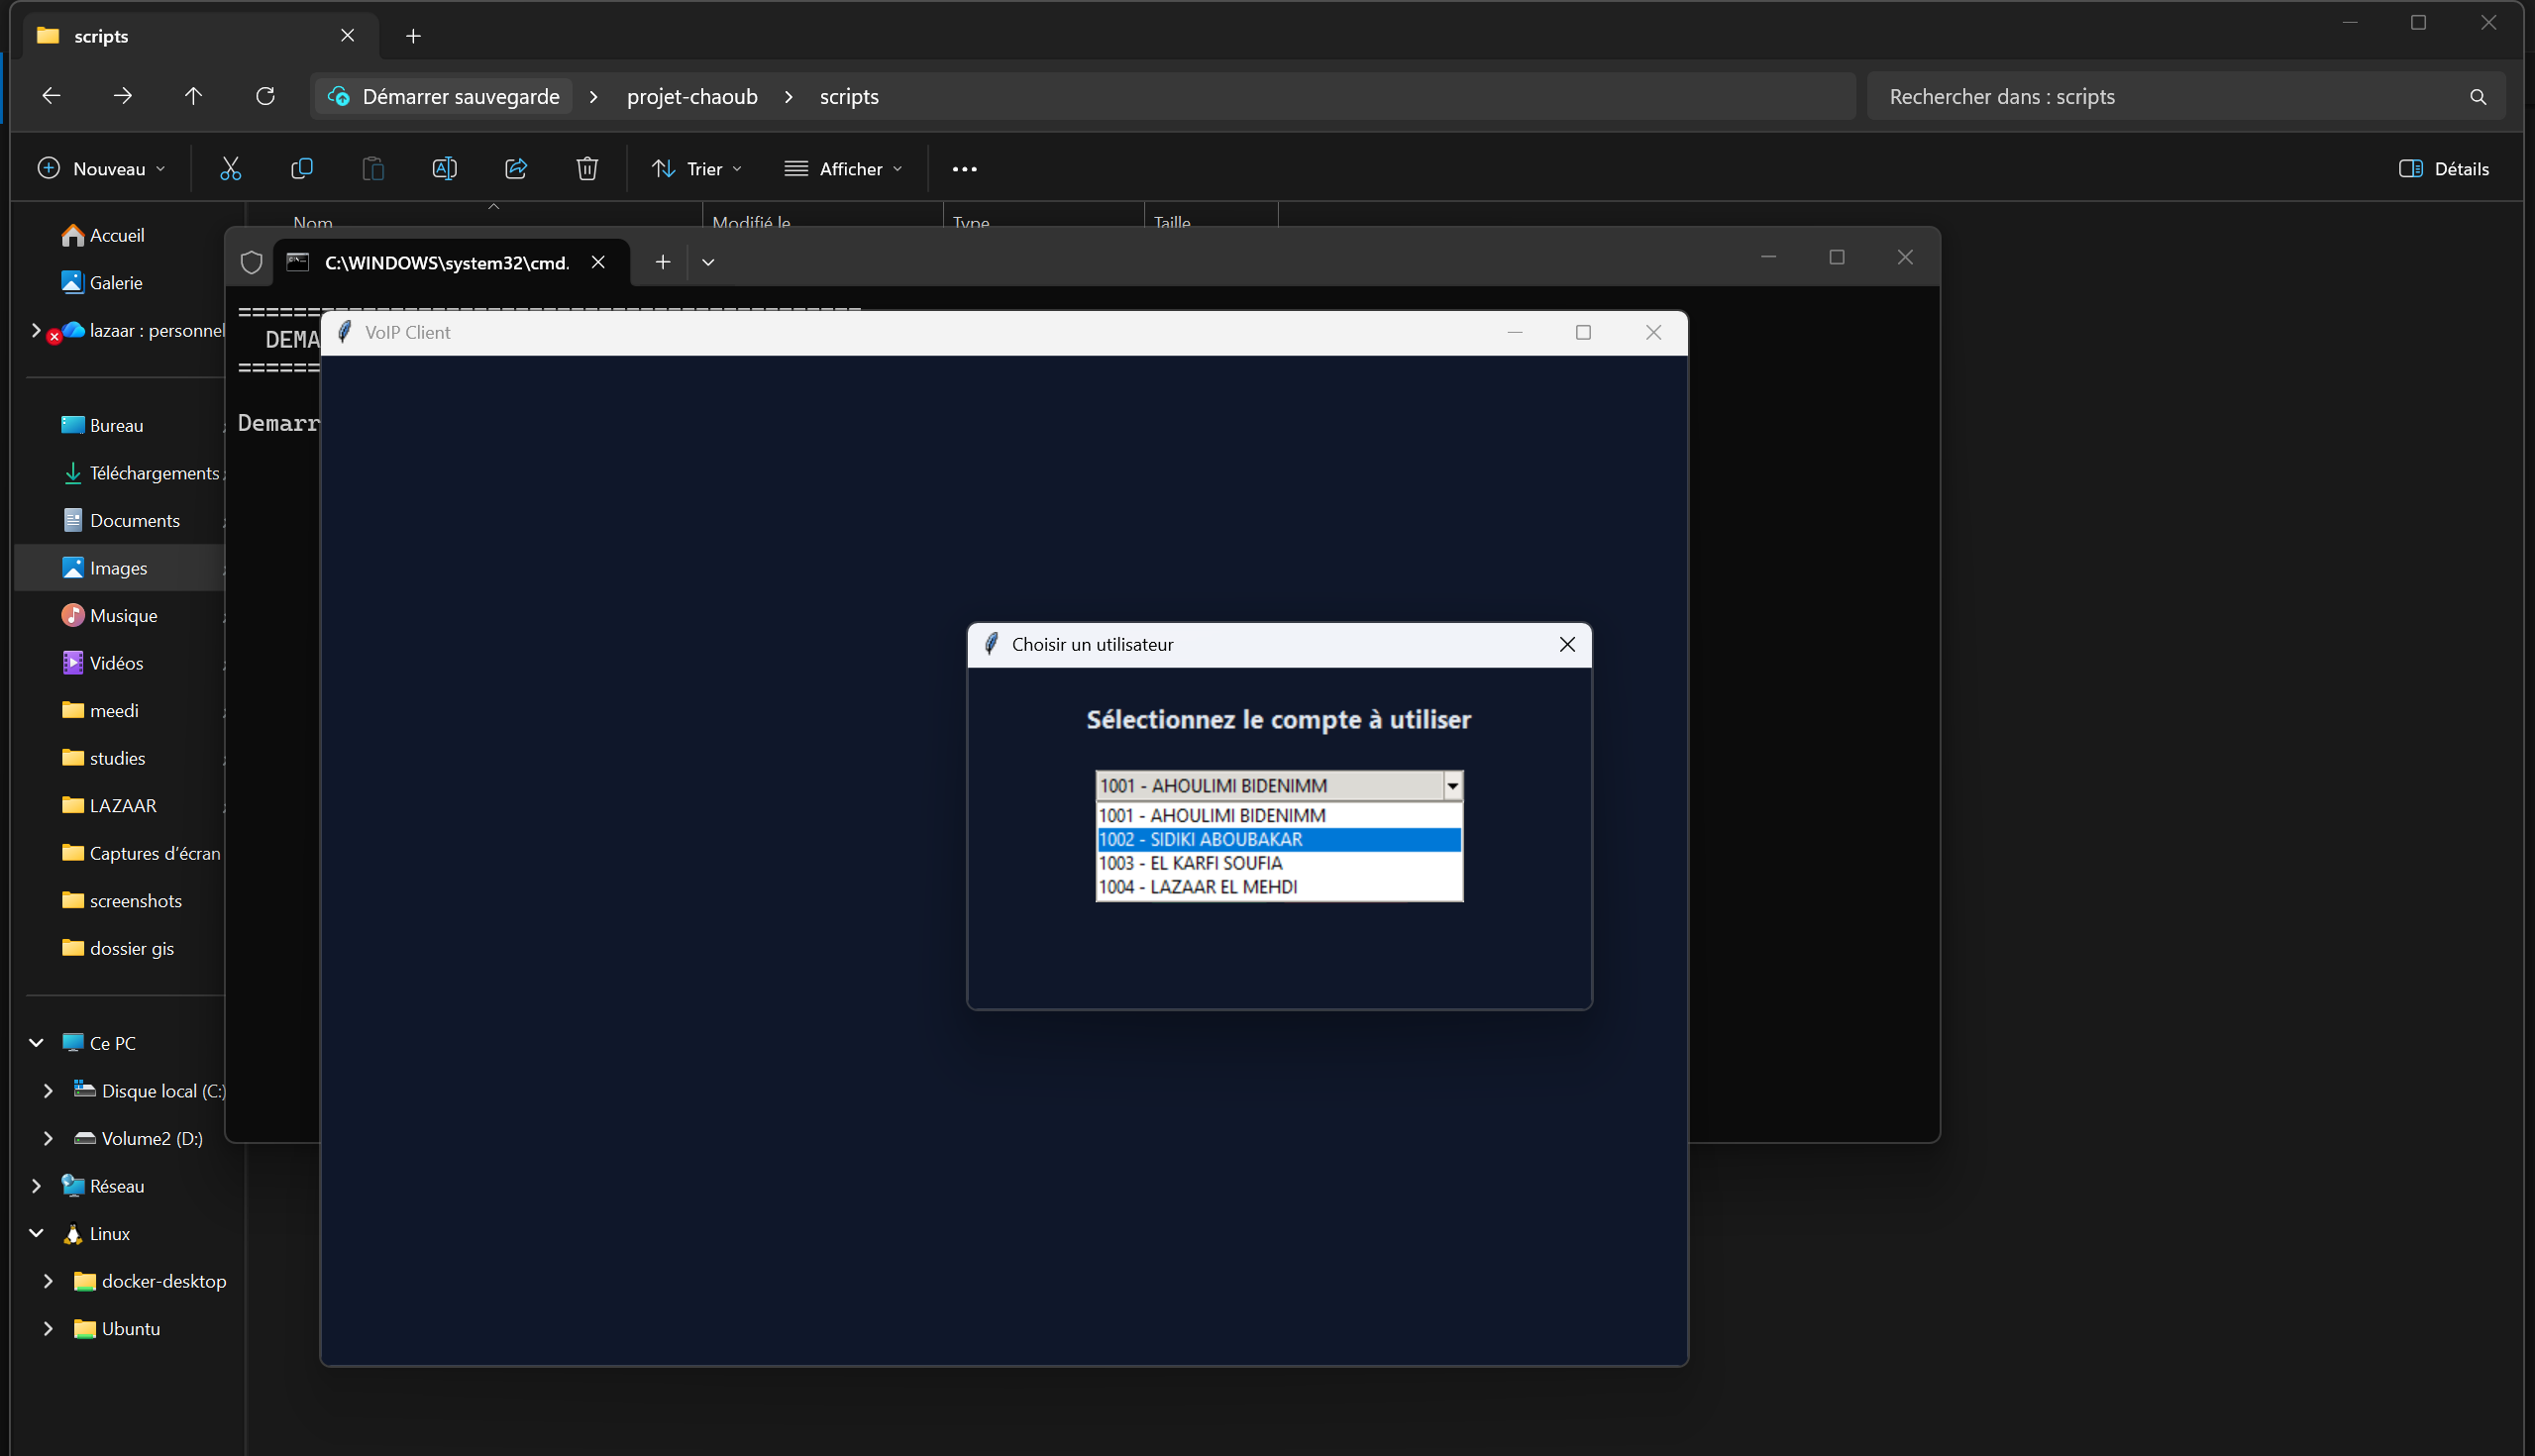
\includegraphics[width=0.8\textwidth]{screenshots/sc5.png}
\end{figure}
\begin{figure}[H]
\centering
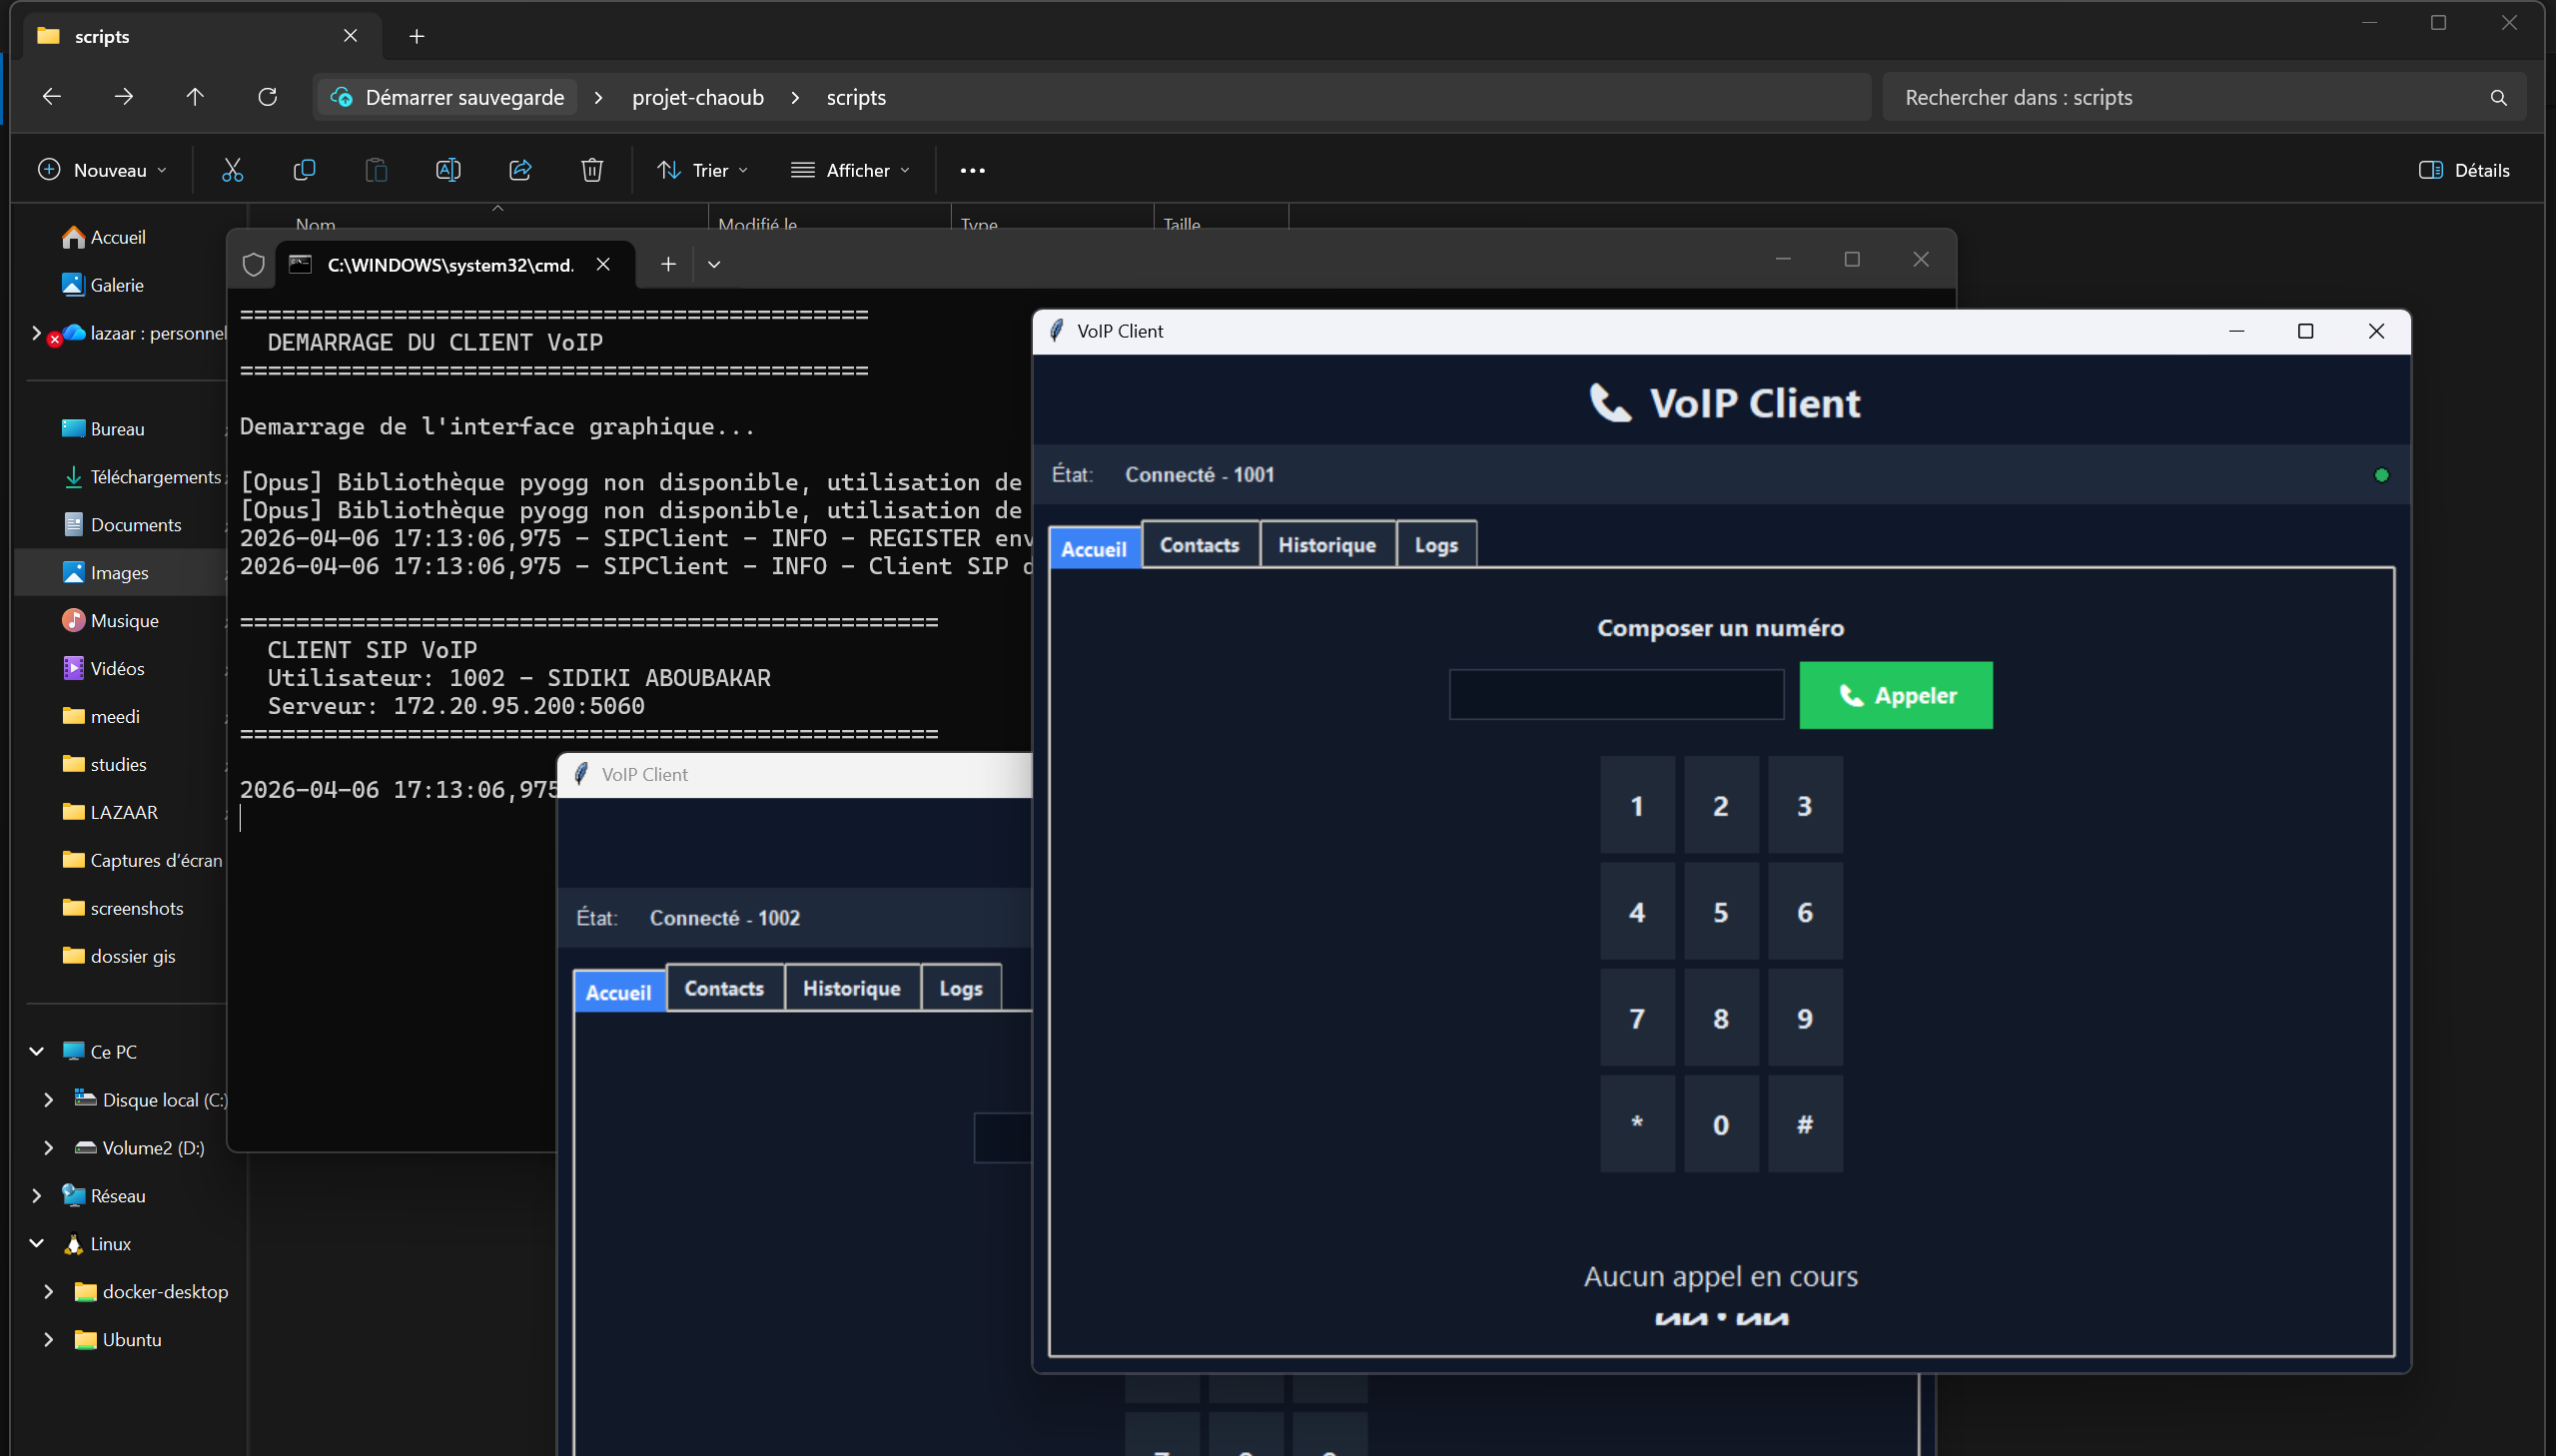
\includegraphics[width=0.8\textwidth]{screenshots/sc6.png}
\end{figure}
\newpage
Etape 3 : Établissement d'un appel et échange audio \\
\begin{figure}[H]
\centering
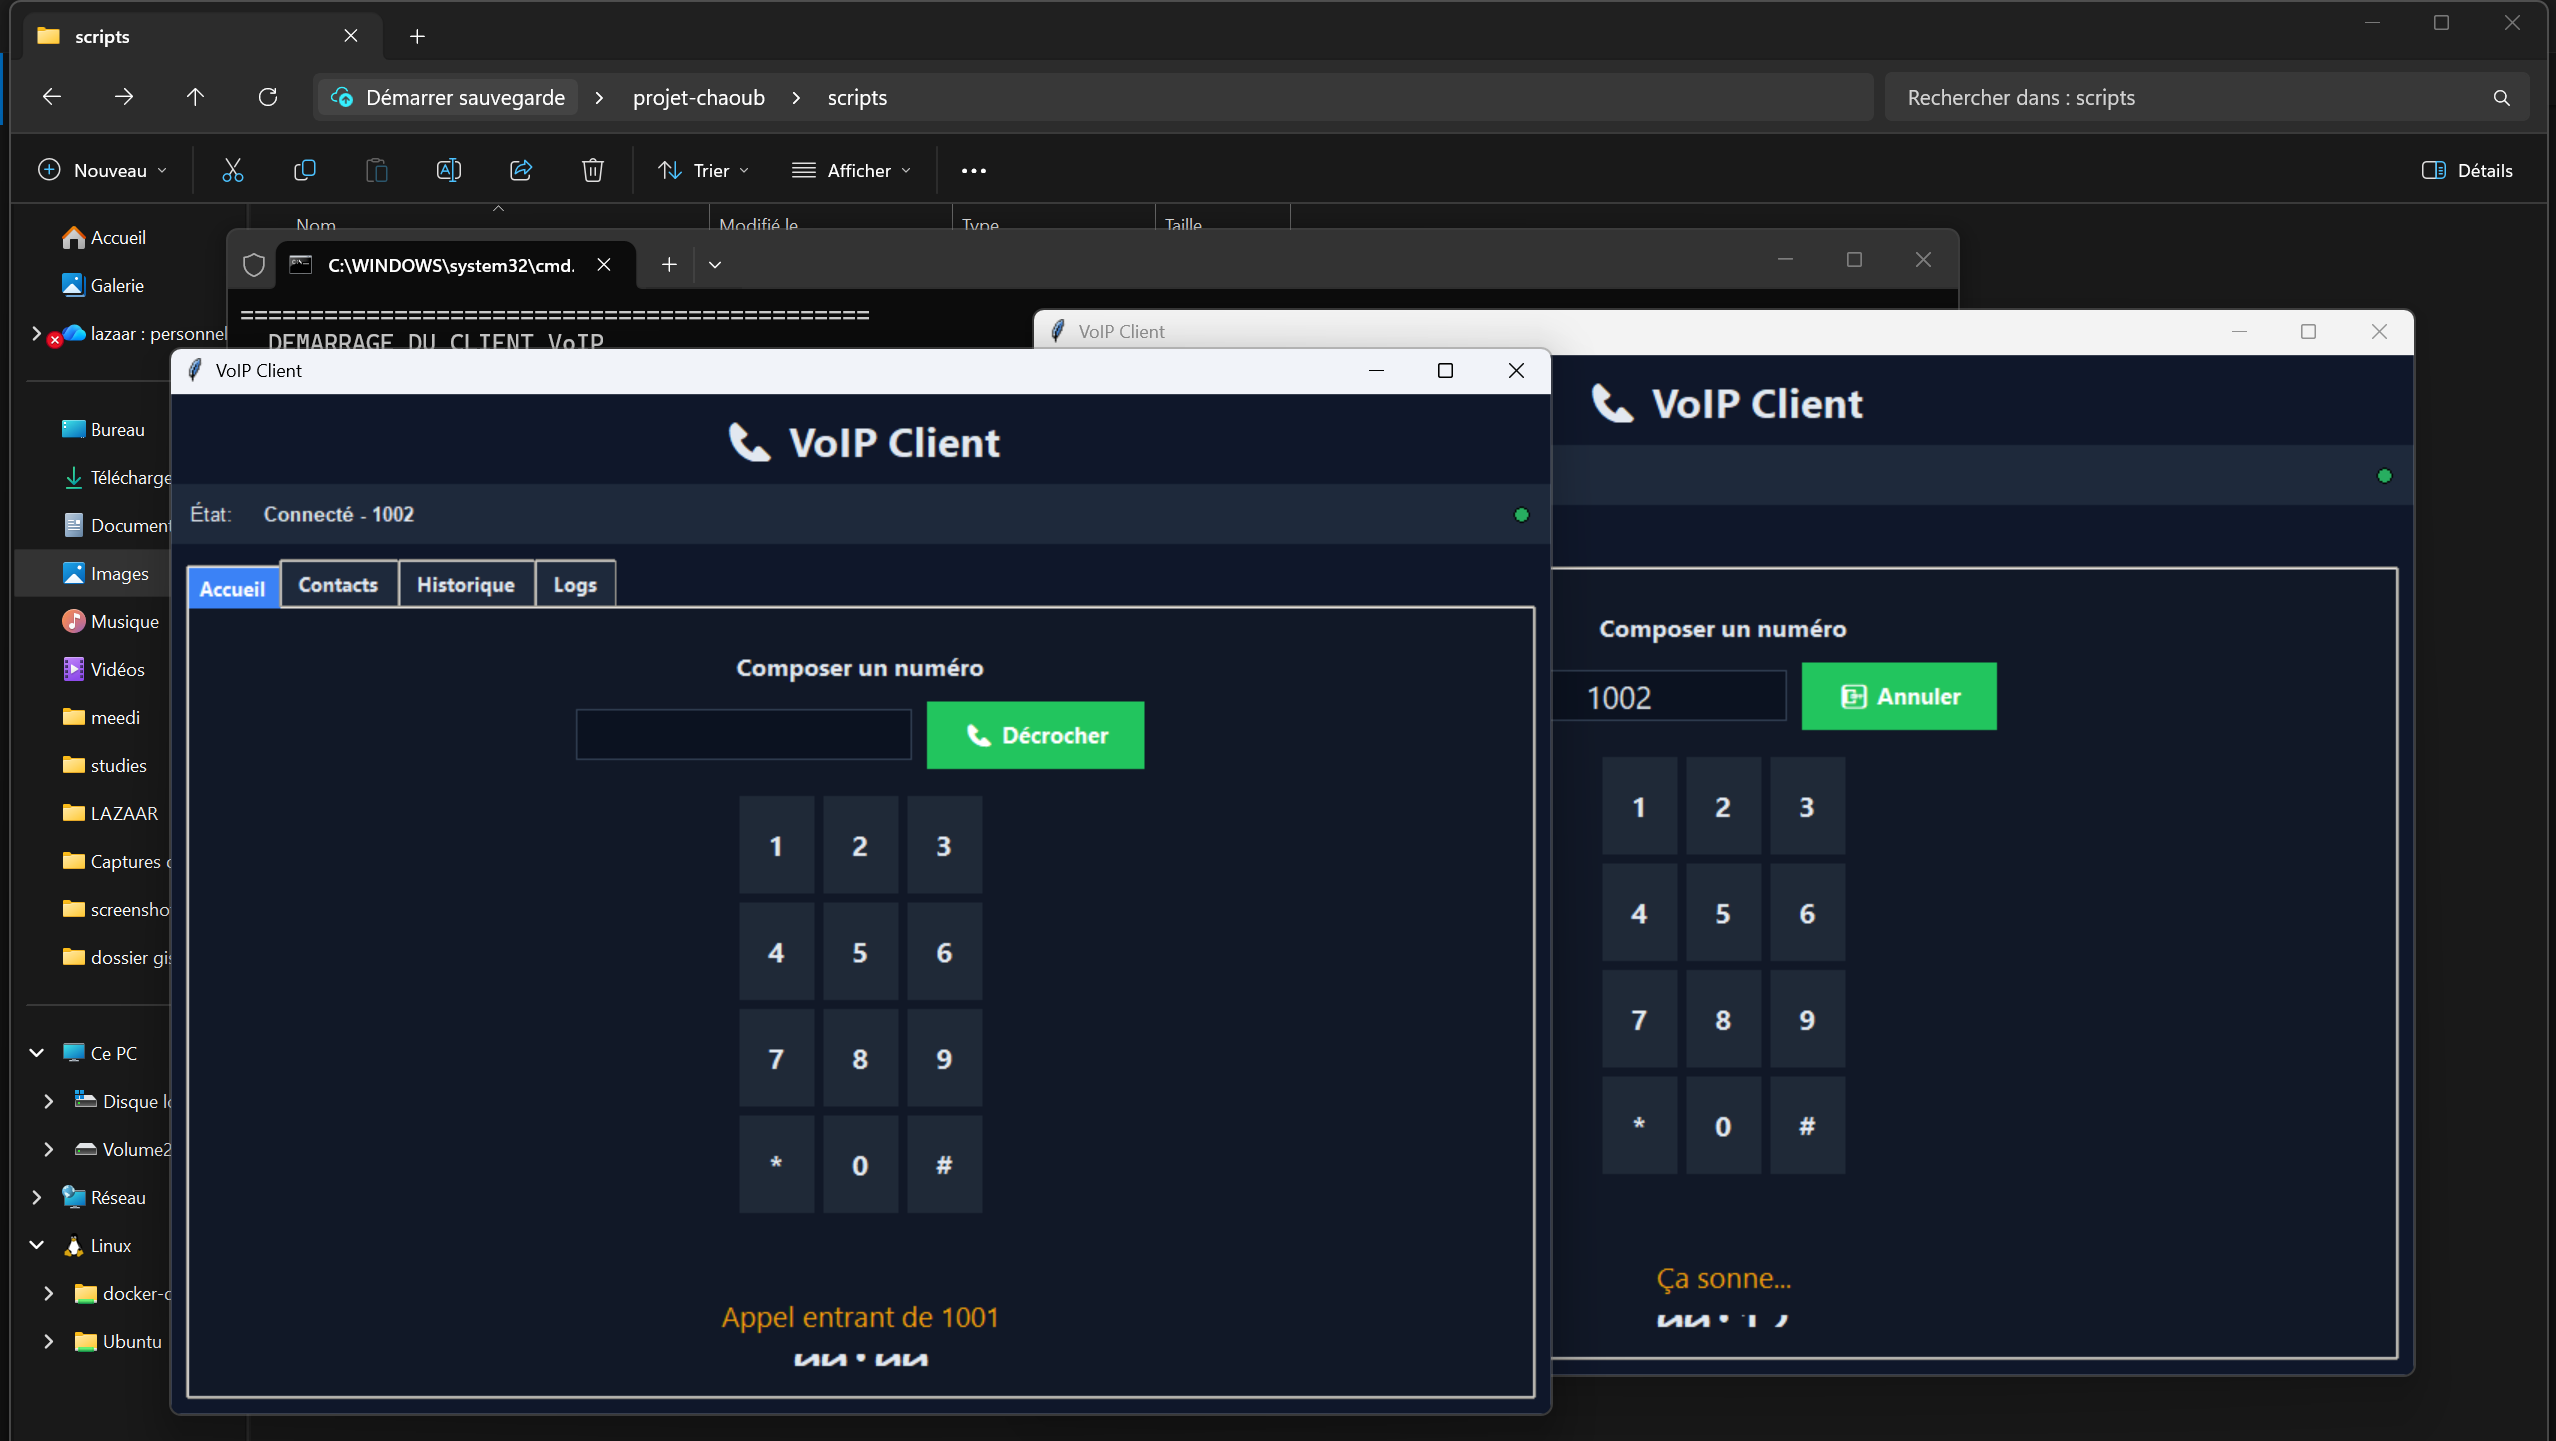
\includegraphics[width=0.8\textwidth]{screenshots/sc7.png}
\end{figure}
\begin{figure}[H]
\centering
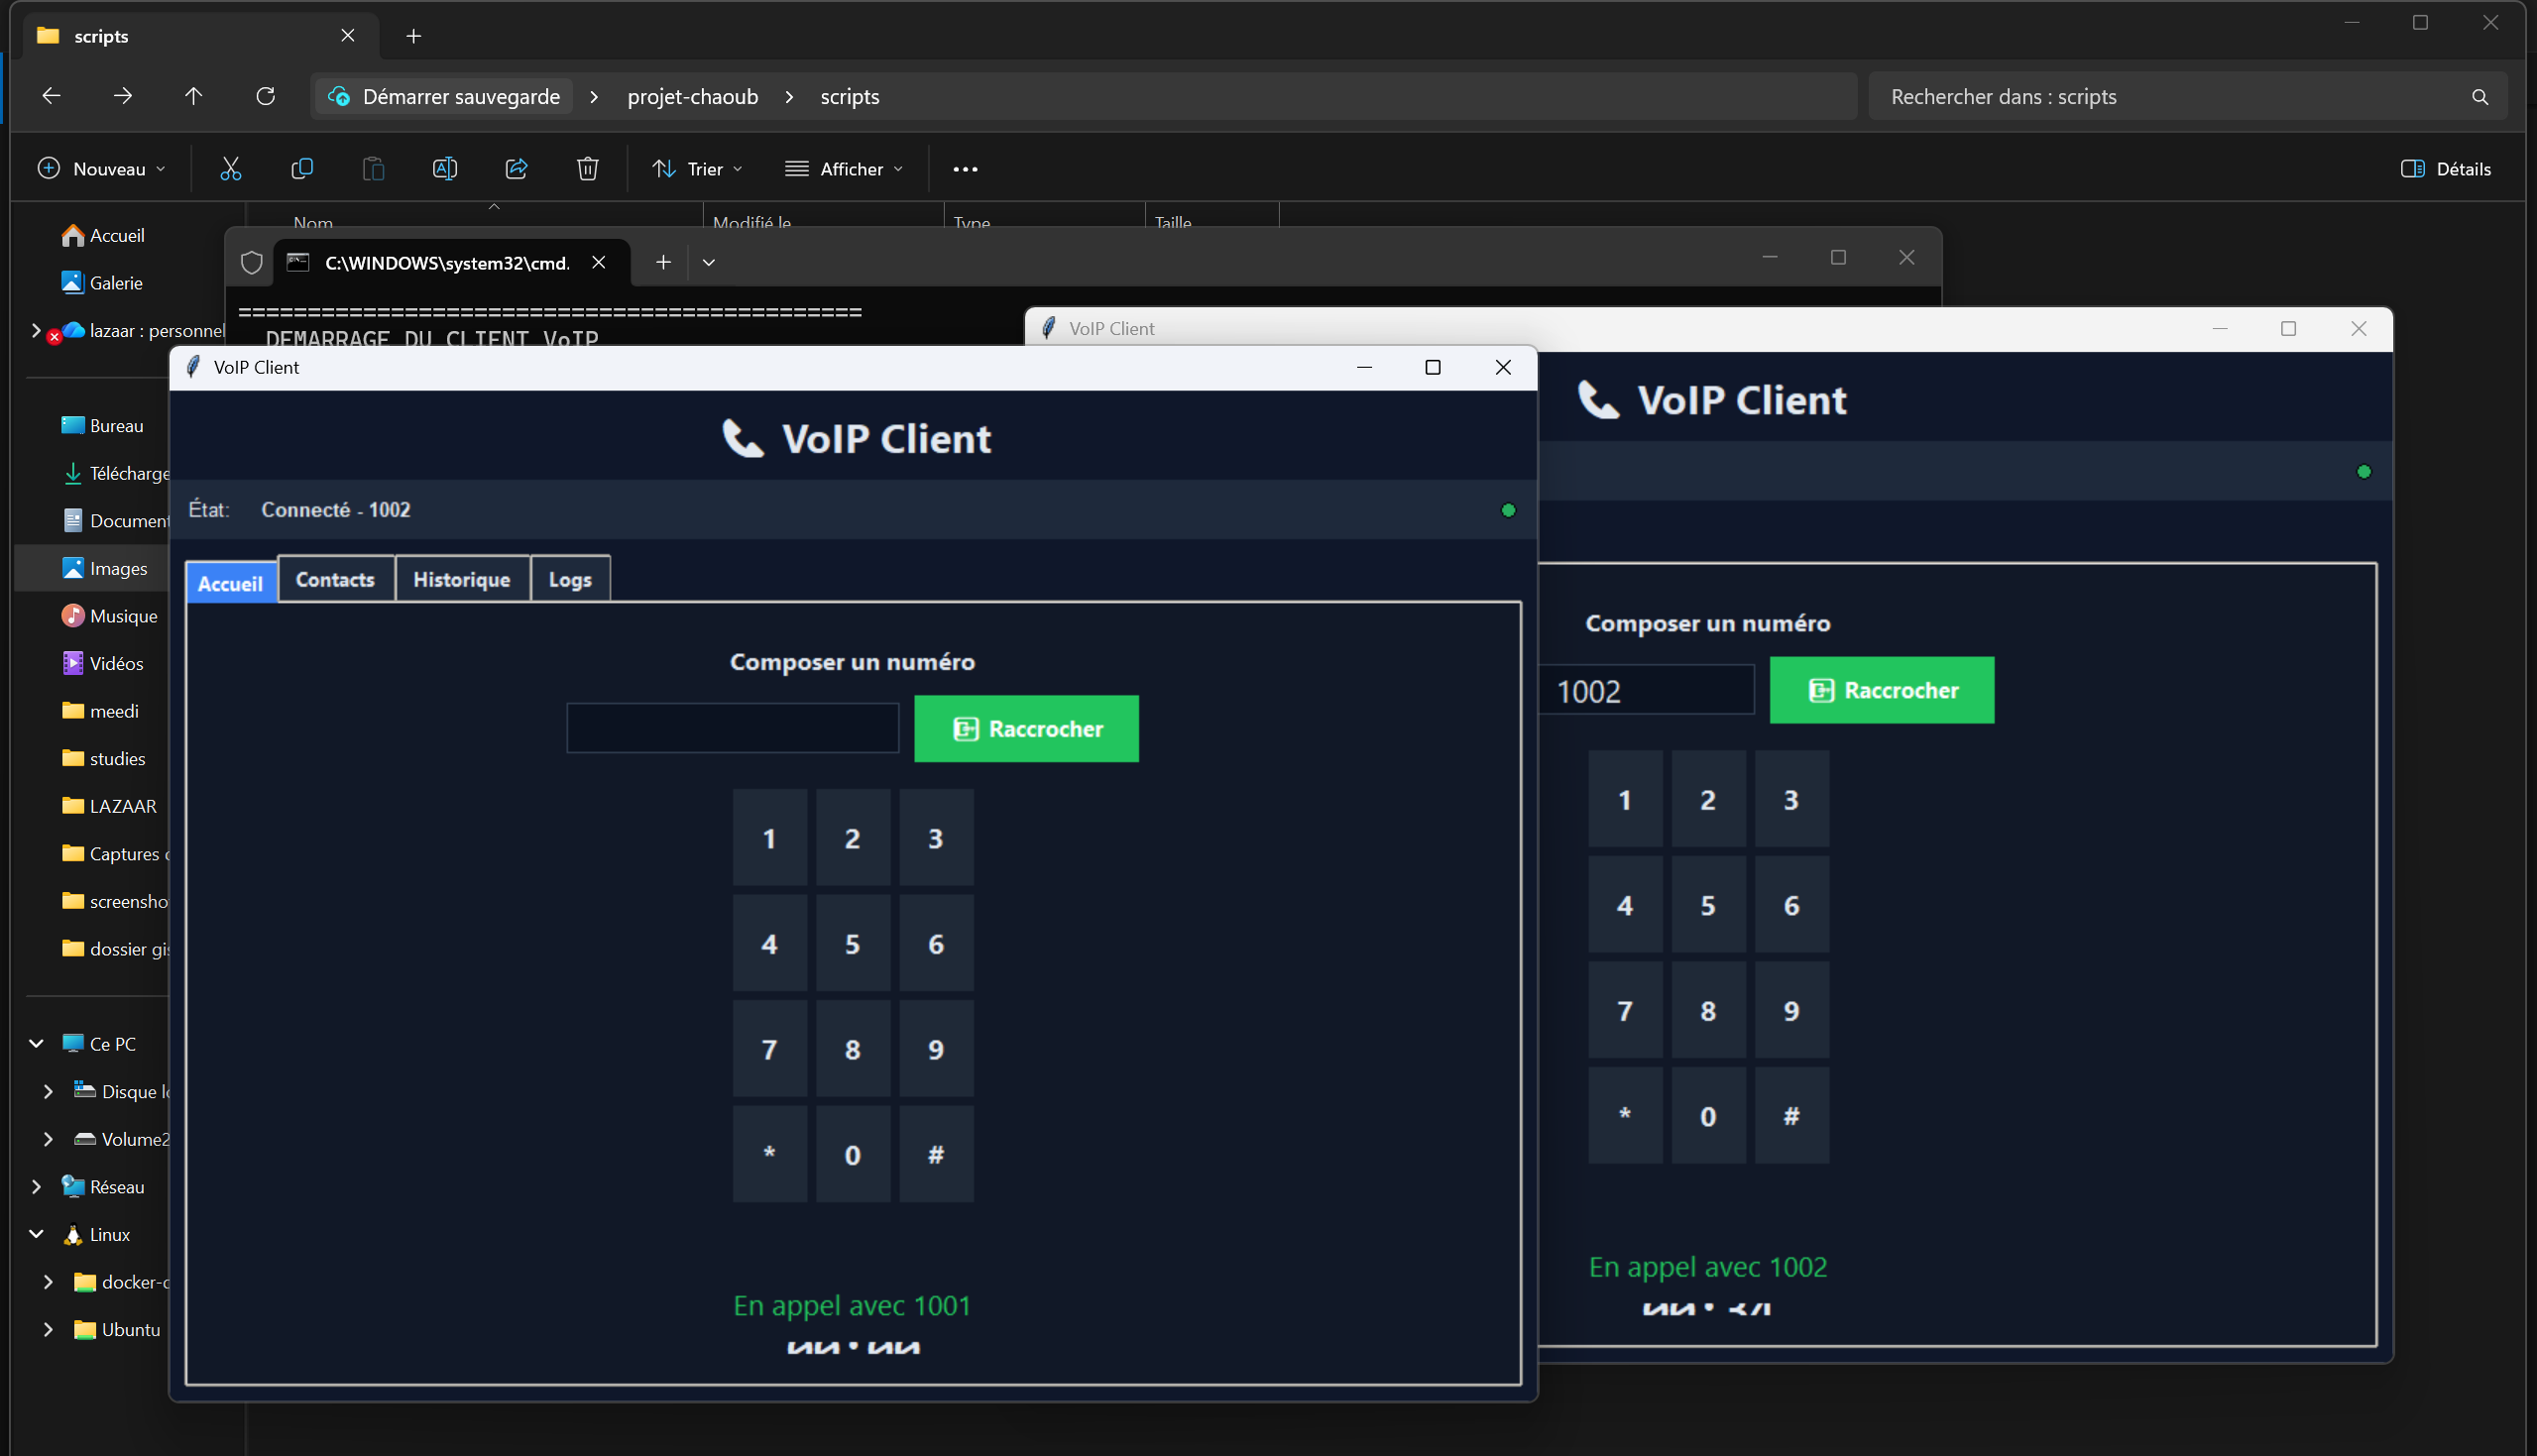
\includegraphics[width=0.8\textwidth]{screenshots/sc8.png}
\end{figure}
\newpage

\section{Tests de connectivité et résultats}

\subsection{Méthodologie de test}

Les validations ont été conduites en deux étapes :
\begin{enumerate}[leftmargin=1.2cm]
    \item tests unitaires audio/codecs/RTP ;
    \item tests de connectivité SIP avec serveur actif.
\end{enumerate}

Scripts utilisés :
\begin{itemize}[leftmargin=1.2cm]
    \item \texttt{tests/test\_audio.py}
    \item \texttt{tests/test\_connectivity.py}
\end{itemize}

\subsection{Résultats obtenus}

\begin{table}[H]
\centering
\begin{tabular}{p{8cm}c}
\toprule
\textbf{Campagne} & \textbf{Résultat} \\
\midrule
Tests audio/codecs/RTP & 5/5 réussis \\
Tests connectivité SIP/SDP/RTP & 7/7 réussis \\
\bottomrule
\end{tabular}
\caption{Synthèse des résultats de test.}
\end{table}

\begin{table}[H]
\centering
\begin{tabular}{p{7cm}p{4cm}p{3cm}}
\toprule
\textbf{Test} & \textbf{Attendu} & \textbf{Statut} \\
\midrule
Serveur SIP accessible (OPTIONS) & Réponse 200 OK & OK \\
REGISTER utilisateur & Enregistrement accepté & OK \\
INVITE vers utilisateur distant & Réponse valide (Trying/Ringing/OK/Not Found) & OK \\
Création/Parsing paquet RTP & Entête + payload cohérents & OK \\
Création/Parsing SDP & IP/Port/Codecs cohérents & OK \\
\bottomrule
\end{tabular}
\caption{Extraits des vérifications fonctionnelles.}
\end{table}

\subsection{Analyse}

Les résultats montrent une cohérence entre la logique de signalisation SIP et la couche média RTP. Le système permet l'enregistrement des clients, l'établissement et la terminaison des appels, ainsi que l'échange audio bidirectionnel. L'ajout d'un support STUN améliore la capacité d'annonce d'endpoint public en environnement NAT, tout en conservant un mode local stable pour les tests en réseau local.

\section{Connexion du système VoIP à Internet : méthodes et choix}

Le passage d'un fonctionnement LAN vers Internet introduit des contraintes supplémentaires : adresses privées non routables, pare-feux d'opérateurs, NAT symétriques et variabilité de latence. Dans ce contexte, la stratégie d'interconnexion doit traiter séparément (i) la signalisation SIP et (ii) le transport média RTP.

\subsection{Méthode 1 : serveur SIP public + redirection de ports}

La première option consiste à héberger le serveur SIP sur une machine publique (VPS ou cloud) avec IP fixe, puis ouvrir les ports nécessaires : UDP 5060 pour SIP et une plage RTP (par exemple 10000--20000).

	\textbf{Avantages :}
\begin{itemize}[leftmargin=1.2cm]
    \item architecture simple à comprendre ;
    \item déploiement rapide pour des démonstrations ;
    \item centralisation de la signalisation.
\end{itemize}

\subsection{Méthode 1 bis : relais RTP côté serveur (implémenté dans ce projet)}

Une extension concrète a été mise en œuvre dans le code du projet : un mode \textbf{relais média côté serveur}. Dans ce mode, le serveur SIP alloue deux ports RTP (un par sens logique), réécrit les SDP de l'offre/réponse, puis relaye les paquets audio entre les deux clients. L'objectif est de contourner les échecs de média direct liés aux NAT restrictifs.

	extbf{Paramètres de configuration associés :}
\begin{itemize}[leftmargin=1.2cm]
    \item \texttt{server.media\_relay\_enabled} : active le relais RTP ;
    \item \texttt{server.public\_host} : IP publique (ou DNS) annoncée dans le SDP ;
    \item \texttt{server.rtp\_port\_start / rtp\_port\_end} : plage de ports relais.
\end{itemize}

	extbf{Avantages :}
\begin{itemize}[leftmargin=1.2cm]
    \item solution immédiatement opérationnelle pour des scénarios Internet contrôlés ;
    \item meilleure tolérance aux topologies NAT difficiles que le pair-à-pair pur ;
    \item cohérence avec une architecture centralisée (serveur SIP déjà présent).
\end{itemize}

	extbf{Limites :}
\begin{itemize}[leftmargin=1.2cm]
    \item consommation de bande passante serveur (audio relayé) ;
    \item absence de négociation ICE complète ;
    \item ne remplace pas TURN/ICE pour une interopérabilité universelle.
\end{itemize}

	\textbf{Limites :}
\begin{itemize}[leftmargin=1.2cm]
    \item le média peut échouer si les deux clients sont derrière des NAT restrictifs ;
    \item la sécurité reste faible sans TLS/SRTP ;
    \item exposition directe des ports sur Internet.
\end{itemize}

\subsection{Méthode 2 : STUN pour découverte d'endpoint public}

STUN (Session Traversal Utilities for NAT) permet au client de découvrir son adresse et port publics, puis d'annoncer ces paramètres dans SDP. Cette approche est déjà partiellement intégrée dans le projet.

	\textbf{Avantages :}
\begin{itemize}[leftmargin=1.2cm]
    \item faible coût d'intégration ;
    \item améliore la réussite des appels pour NAT de type full-cone ou restricted-cone ;
    \item conserve un chemin média direct (latence souvent meilleure).
\end{itemize}

	\textbf{Limites :}
\begin{itemize}[leftmargin=1.2cm]
    \item insuffisant face aux NAT symétriques/CGNAT ;
    \item pas de garantie de connectivité universelle ;
    \item dépendance à des serveurs STUN externes.
\end{itemize}

\subsection{Méthode 3 : ICE + TURN (approche robuste recommandée)}

ICE (Interactive Connectivity Establishment) orchestre plusieurs candidats réseau (hôte local, réflexif STUN, relayé TURN) et choisit automatiquement le meilleur chemin. TURN relaie le média lorsque le pair-à-pair est impossible.

	\textbf{Avantages :}
\begin{itemize}[leftmargin=1.2cm]
    \item taux de réussite élevé en environnement Internet réel ;
    \item robustesse face aux NAT complexes ;
    \item meilleure expérience utilisateur (moins d'échecs silencieux).
\end{itemize}

	\textbf{Coûts/contraintes :}
\begin{itemize}[leftmargin=1.2cm]
    \item complexité d'implémentation plus importante ;
    \item besoin d'un serveur TURN dimensionné (bande passante et coût) ;
    \item logique de sélection/monitoring des candidats à intégrer côté client.
\end{itemize}

\subsection{Méthode 4 : VPN inter-sites}

Une alternative pragmatique en contexte académique consiste à placer les deux clients dans un même réseau logique via VPN (WireGuard/OpenVPN). L'application se comporte alors comme en LAN.

	\textbf{Avantages :}
\begin{itemize}[leftmargin=1.2cm]
    \item mise en œuvre souvent plus simple qu'ICE/TURN complet ;
    \item bon niveau de sécurité si le VPN est bien configuré ;
    \item évite l'exposition directe des ports SIP/RTP au public.
\end{itemize}

	\textbf{Limites :}
\begin{itemize}[leftmargin=1.2cm]
    \item nécessite l'installation/gestion d'une infrastructure VPN ;
    \item moins adapté à un service grand public ;
    \item dépendance opérationnelle au tunnel VPN.
\end{itemize}

\subsection{Choix recommandés selon le contexte}

\begin{table}[H]
\centering
\begin{tabular}{p{4.3cm}p{5.2cm}p{4.5cm}}

    oprule
	\textbf{Contexte} & \textbf{Choix recommandé} & \textbf{Justification} \\
\midrule
Prototype local/LAN & SIP serveur local + RTP direct & Simplicité, faible latence, débogage rapide \\
\midrule
Démo Internet contrôlée & Serveur SIP public + relais RTP + STUN & Déploiement réalisable rapidement sur 2 PC distants \\
\midrule
Production multi-opérateurs & SIP public + ICE + TURN + TLS/SRTP & Meilleure robustesse et sécurité \\
\midrule
Usage académique distant & VPN + serveur SIP interne & Déploiement stable sans exposition publique forte \\
\bottomrule
\end{tabular}
\caption{Comparaison des stratégies de connexion Internet pour la solution VoIP.}
\end{table}

\subsection{Plan d'évolution proposé pour ce projet}

Pour rendre l'application durablement opérationnelle entre deux PC distants sur Internet, la trajectoire la plus pertinente devient :
\begin{enumerate}[leftmargin=1.2cm]
    \item conserver le mode relais RTP serveur comme base fonctionnelle initiale ;
    \item déployer le serveur SIP sur un hôte public avec IP fixe (ou DNS) ;
    \item sécuriser la signalisation (SIP over TLS) et le média (SRTP) ;
    \item intégrer un mécanisme ICE/TURN pour améliorer l'interopérabilité globale ;
    \item instrumenter des métriques de qualité (latence, gigue, pertes) pour pilotage adaptatif.
\end{enumerate}

Cette progression conserve la base actuelle du projet tout en améliorant progressivement l'interopérabilité Internet, la sécurité et la fiabilité des appels.

\section{Conclusion}

Ce projet démontre la réalisation complète d'une chaîne VoIP académique basée sur des standards ouverts. L'architecture mise en place confirme la séparation claire entre signalisation (SIP/SDP) et média (RTP), ainsi que la pertinence d'un serveur SIP léger pour l'orchestration des appels.

Sur le plan pédagogique, les objectifs sont atteints : compréhension des protocoles, implémentation opérationnelle, tests reproductibles, et interface utilisateur exploitable. Les perspectives d'amélioration incluent :
\begin{itemize}[leftmargin=1.2cm]
    \item intégration ICE/TURN complète pour traversée NAT avancée,
    \item sécurisation média (SRTP) et signalisation (TLS),
    \item enrichissement des métriques de qualité (gigue, perte, MOS estimé),
    \item extension vers des conférences multi-participants.
\end{itemize}


\begin{thebibliography}{9}
\bibitem{rfc3261}
J. Rosenberg et al., \textit{SIP: Session Initiation Protocol}, RFC 3261, IETF, 2002.

\bibitem{rfc3550}
H. Schulzrinne et al., \textit{RTP: A Transport Protocol for Real-Time Applications}, RFC 3550, IETF, 2003.

\bibitem{rfc4566}
M. Handley et al., \textit{SDP: Session Description Protocol}, RFC 4566, IETF, 2006.

\bibitem{webrtc}
A. Bergkvist et al., \textit{WebRTC 1.0: Real-time Communication Between Browsers}, W3C Recommendation.
\end{thebibliography}

\end{document}
